\documentclass[conference]{IEEEtran}
% Draft v0 (Nov 22, 2026). Built from docs/report/report.tex, docs/report/report_ppo.tex and
% docs/planner_{A,B,C}.md on origin/main. Red \todo{} notes mark what the team still has to decide or check.

\usepackage{cite}
\usepackage{amsmath,amssymb}
\usepackage{graphicx}
\usepackage{booktabs}
\usepackage{array}
\usepackage{multirow}
\usepackage{xcolor}
\usepackage{tikz}
\usetikzlibrary{arrows.meta,positioning,calc,fit,patterns}
\usepackage{pgfplots}
\pgfplotsset{compat=1.18}
\usepackage{algorithm}
\usepackage{algpseudocode}
\usepackage[hidelinks]{hyperref}

\newcommand{\todo}[1]{\textcolor{red}{[TODO: #1]}}
\newcommand{\repo}{https://github.com/Shivsi7/dynamic-grasping/blob/main}
\newcommand{\vid}[1]{\href{\repo/docs/report/videos/#1.mp4}{video}}
\newcommand{\sg}{\operatorname{sg}}

\begin{document}

\title{Teaching A Robot Arm To Pick Up And Dodge}

\author{\IEEEauthorblockN{Eli Olcott, Victor Conchello Vendrell, Shivam Singhal}
\IEEEauthorblockA{6.4212 Robotic Manipulation, Fall 2026}}

\maketitle

% ---------------------------------------------------------------------------------------------------
\begin{abstract}
Picking an object off a moving conveyor is routine when the workspace is empty, but robots increasingly
share their workspace with other moving things: people, objects, and other robots. So, the arm must be able to reach a moving target while
staying clear of obstacles that are themselves in motion. We study this problem in simulation with a
7-DoF KUKA iiwa and a WSG gripper that must grasp a YCB object from a moving cart while up to four
obstacles cross the workspace. We implement four controllers on a shared harness: a reactive QP with
velocity dampers, a space-time RRT-Connect planner, a space-time kinematic trajectory optimizer, and a
neural policy trained by behavior cloning, DAgger and PPO from the optimizer's demonstrations. All are
evaluated on 214 scenes under a protocol in which computation time costs simulated time and an episode
only counts as a success if the object is still held when the scene ends. Trajectory optimization
succeeds in 91\% of scenes, the learned policy in 90\% at about 1/1200 of the optimizer's compute, the
space-time planner in 81\% with no collisions, and the reactive controller in 62\%. The results show a
trade-off between safety, success and compute: deliberative planning is safest, optimization reaches
the most grasps, and a distilled policy recovers most of the optimizer's success in real time but
collides more often in unseen scenes.
\end{abstract}

% ---------------------------------------------------------------------------------------------------
\section{Introduction}

Robots that pick from conveyors, hand over objects to people, or work beside other machines must grasp
objects that are moving, in workspaces where other things are moving too. Both motions constrain the
arm at once: it has to arrive at the object at the right place \emph{and} time, and it must not be
anywhere an obstacle will be at the time it is there. A static plan computed for a frozen snapshot of
the scene is not enough, and neither is a plan that ignores how long it took to compute it, since the
scene keeps moving during that time.

We consider the following task (Fig.~\ref{fig:teaser}). A KUKA iiwa with a Schunk WSG gripper must
pick one of six YCB objects~\cite{calli2015ycb} off a carrier riding a conveyor at
0.05--0.3\,m/s, while zero to four obstacles (spheres and boxes on wheeled rigs, or free-flying lobbed
shapes) cross the workspace at up to 0.5\,m/s. The motion of the cart and obstacles is known in
advance; we discuss relaxing this with perception in Section~\ref{sec:conclusion}.

\begin{figure*}[t]
  \centering
  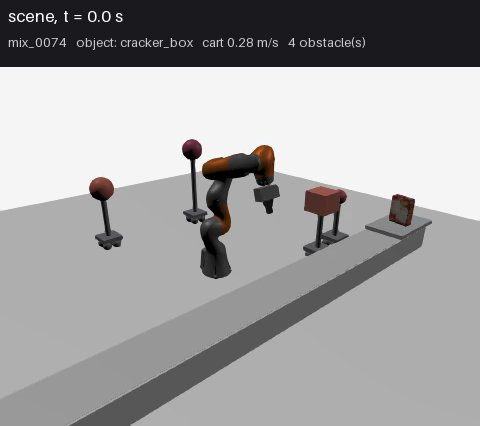
\includegraphics[width=0.245\textwidth]{frames/mix_0074_0.jpg}\hfill
  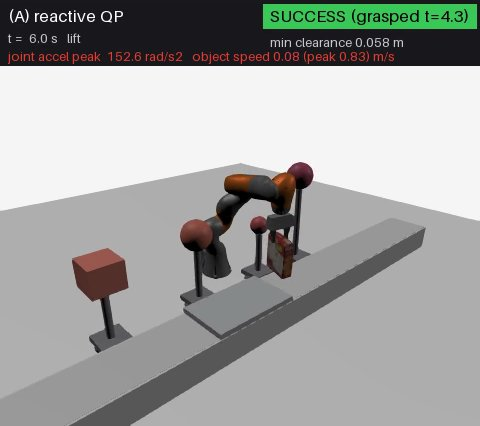
\includegraphics[width=0.245\textwidth]{frames/mix_0074_1.jpg}\hfill
  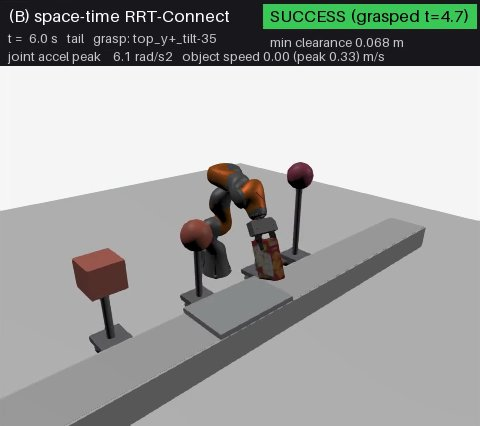
\includegraphics[width=0.245\textwidth]{frames/mix_0074_2.jpg}\hfill
  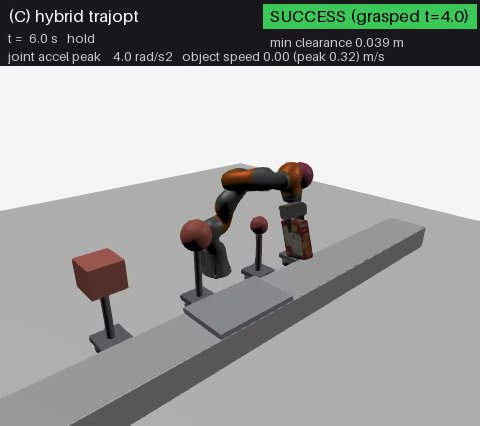
\includegraphics[width=0.245\textwidth]{frames/mix_0074_3.jpg}
  \caption{The task. A cracker box rides a moving carrier past the iiwa while four obstacles on wheeled
  rigs cross the workspace (left, $t=0$). The other panels show the reactive controller (A), the
  space-time planner (B) and the trajectory optimizer (C) each grasping the box in held-out scene
  \texttt{mix\_0074}, 1.0 to 1.7\,s after it comes into reach (\vid{mix_0074}).}
  \label{fig:teaser}
\end{figure*}

\textbf{Design goals.} A controller for this task should
(G1) grasp and lift the object and still hold it when the scene ends;
(G2) never touch an obstacle, the cart or the floor;
(G3) command motion the real arm could execute, within its velocity, acceleration and torque limits; and
(G4) do so in real time, with its own computation counted against the clock.
\todo{agree on concrete target values for G1--G4, e.g.\ $\ge 85\%$ success, zero collisions, peak torque below the limit, $\le 100$\,ms per decision.}

\textbf{Approach.} These goals pull in different directions, and the classic families of methods resolve
them differently. We therefore implement four controllers on one shared harness and compare them on the
same 214 scenes: (A) a reactive QP controller that never plans; (B) a space-time RRT-Connect planner that
replans every 0.5\,s; (C) a space-time trajectory optimizer that plans the whole grasp; and (D) a neural
policy distilled from (C) and fine-tuned with reinforcement learning. A naive controller that ignores the
obstacles serves as a baseline.

\textbf{Contributions.}
\begin{itemize}
  \item A benchmark for dynamic grasping among moving obstacles in Drake: a seeded scene generator, three
    preset grids that block the direct grasp, and an evaluation protocol in which compute time costs
    simulated time and success requires holding the object to the end of the scene.
  \item Four controllers built on the same world model and harness: a velocity-damper QP, a space-time
    RRT-Connect planner with acceleration-aware extensions and escape moves, an IK-seeded space-time
    trajectory optimizer, and a BC$\to$DAgger$\to$PPO policy.
\end{itemize}

% ---------------------------------------------------------------------------------------------------
\section{Related Work}

\textbf{Dynamic grasping.} Early work tracked and grasped a moving object with a visual servoing loop
on a hand-eye system~\cite{allen1993tracking}. Marturi et al.~\cite{marturi2019dynamic} plan grasps and
trajectories for objects moving along unknown paths, and Akinola et al.~\cite{akinola2021dynamic}
choose grasps by reachability and the object's motion, replanning as the object moves. These works
focus on the target and assume a free workspace. We add obstacles that move as well, which makes
\emph{when} the arm is somewhere as important as where.

\textbf{Planning among moving obstacles.} Velocity obstacles~\cite{fiorini1998velocity} reason about
collisions in velocity space for agents with simple shapes. Sampling-based planners handle
high-dimensional arms; RRT-Connect~\cite{kuffner2000rrtconnect} grows two trees toward each other in
configuration space, and ST-RRT*~\cite{grothe2022strrt} extends bidirectional search to space-time,
with time as an unbounded dimension, velocity-bounded edges and sampling restricted to the states
reachable in time. Planner (B) follows ST-RRT*'s formulation but searches for the first feasible path
to one of many timed goals, replans continuously, and adds acceleration constraints so that the result
is executable. VAMP~\cite{thomason2024vamp} shows that vectorized collision checking can make sampling
planners run in microseconds, which would let a planner like (B) replan at control rates; we did not
adopt it, and collision checking remains (B)'s bottleneck.

\textbf{Reactive control.} Potential fields~\cite{khatib1986realtime} and velocity
dampers~\cite{faverjon1987local} keep a manipulator away from obstacles inside the control loop.
NEO~\cite{haviland2021neo} combines velocity dampers with a differential-IK quadratic program for
reactive manipulation among obstacles. These methods run at kilohertz rates but are local: they can
stall behind an obstacle that must be gone around. Controller (A) is in this family, with dampers
against the obstacles' predicted swept volume.

\textbf{Trajectory optimization.} CHOMP~\cite{ratliff2009chomp} and TrajOpt~\cite{schulman2014trajopt}
optimize whole trajectories against collision costs or constraints, and Drake's kinematic trajectory
optimization~\cite{tedrake2019drake,tedrake2024manipulation} optimizes B-spline trajectories with free
duration under general constraints, solved with SNOPT~\cite{gill2005snopt}. Such methods produce smooth,
time-optimal motion but are sensitive to their initial guess and give no guarantee on solve time.
Controller (C) seeds the optimizer with collision-aware IK and evaluates collision constraints at the
time the trajectory reaches each point.

\textbf{Learning motion from planners.} Motion Policy Networks~\cite{fishman2022mpinets} train a neural
policy on millions of trajectories from a global planner and run faster than the planners they imitate.
DAgger~\cite{ross2011dagger} corrects the distribution shift of behavior cloning by labeling the
learner's own states with an expert, and PPO~\cite{schulman2017ppo} with generalized advantage
estimation~\cite{schulman2016gae} fine-tunes a policy on its own reward. Policy (D) combines all three,
with (C) as the expert.

Taken together, these families trade completeness, speed and smoothness differently, and none of the
works above compares them on the same dynamic grasping task under the same compute budget. That is the
gap this project fills.

% ---------------------------------------------------------------------------------------------------
\section{Problem Formulation}
\label{sec:problem}

\textbf{Scene.} The world frame has the iiwa base at the origin. A conveyor runs along $y$ at
$x\approx0.63$\,m; its carrier (top at $z=0.20$\,m) moves at a constant speed in $[0.05, 0.30]$\,m/s,
enters the robot's reach ($|y|<0.5$\,m) at $t=3$\,s and stays in reach for $1/\text{speed}$ seconds.
The target is one of six YCB objects (soup can, sugar box, gelatin box, potted meat can, cracker box,
mustard bottle), standing free on the carrier. Obstacles are spheres (radius 5--10\,cm) or boxes
(10--20\,cm) on masts of wheeled rigs moving at 0.1--0.5\,m/s through the corridor between the robot
and the conveyor or beside the robot, or free-flying shapes on ballistic paths. Obstacle paths are timed
to cross while the target is reachable, but never hit the conveyor, the robot's base or each other, so
every scene can be solved by getting out of the way. Obstacles are dynamic bodies driven by stiff
PD joints, so collisions are physical.

\textbf{Information.} A controller sees the robot's measured state $(q, \dot q)$ and gripper width,
and a \emph{world model} that predicts the pose and velocity of the target, the cart and every
obstacle at any time $t$. In this work the prediction is exact.

\textbf{Commands.} A controller runs every 10\,ms (5\,ms for (C), 0.1\,s for (D)) and returns joint positions,
joint velocities or a time-indexed joint trajectory, plus a gripper opening.

\textbf{Computation costs time.} The simulator waits for the controller, so by default a slow
controller would look instantaneous. Instead, a command computed in $w$ seconds of wall time takes
effect $w$ seconds of simulated time later; the previous command keeps executing meanwhile. A
trajectory that would make the arm jump when it takes effect (more than 0.02\,rad from the executing
one) is rejected. This \emph{measured latency} makes compute speed part of the result.

\textbf{Outcomes.} An episode ends in one of four outcomes. A \emph{collision} is any contact between
a robot link and an obstacle, the cart, the floor or the target (other than the gripper touching the
target); it takes precedence. \emph{Success} requires the object to be in hand and at least 5\,cm above
its rest height for 0.5\,s, and still in hand and lifted when the scene ends: episodes are simulated
to the end of the scene, so a controller that grasps and then flings or drops the object does not
score. Otherwise the outcome is \emph{dropped} (lifted, then lost) or \emph{timeout}.

\textbf{Assumptions.} Perfect state and perfect prediction of all motion; known object identity and
geometry; a position-controlled arm as in the course's hardware station~\cite{tedrake2024manipulation};
simulation only.

% ---------------------------------------------------------------------------------------------------
\section{Approach}
\label{sec:approach}

Fig.~\ref{fig:architecture} shows the shared system. All four controllers plug into the same
\texttt{Controller} interface, read the same world model, and query the same collision geometry: a
kinematic copy of the Drake scene in which every obstacle, the cart and the target are placed at their
predicted poses at a queried time $t$, so that signed distances between the robot at $q$ and the world
at $t$ are available for any $(q, t)$.

\begin{figure}[t]
  \centering
  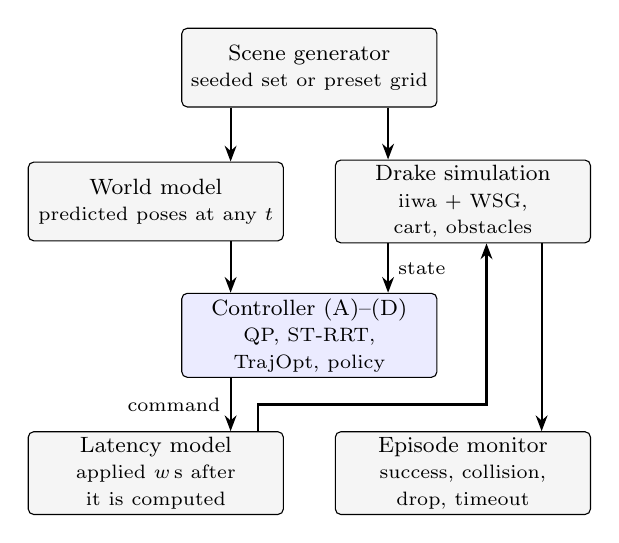
\begin{tikzpicture}[
      font=\footnotesize,
      box/.style={draw, rounded corners=2pt, align=center, text width=3.1cm, minimum height=10mm, inner sep=2pt, fill=gray!8},
      arr/.style={-{Stealth[length=2mm]}, thick}]
    \node[box] (gen) at (0,0) {Scene generator\\{\scriptsize seeded set or preset grid}};
    \node[box] (wm) at (-1.95,-1.7) {World model\\{\scriptsize predicted poses at any $t$}};
    \node[box] (sim) at (1.95,-1.7) {Drake simulation\\{\scriptsize iiwa + WSG, cart, obstacles}};
    \node[box, fill=blue!8] (ctrl) at (0,-3.4) {Controller (A)--(D)\\{\scriptsize QP, ST-RRT, TrajOpt, policy}};
    \node[box] (mon) at (1.95,-5.15) {Episode monitor\\{\scriptsize success, collision, drop, timeout}};
    \node[box] (lat) at (-1.95,-5.15) {Latency model\\{\scriptsize applied $w$\,s after it is computed}};
    \draw[arr] ([xshift=-10mm]gen.south) -- ([xshift=-10mm]gen.south |- wm.north);
    \draw[arr] ([xshift=10mm]gen.south) -- ([xshift=10mm]gen.south |- sim.north);
    \draw[arr] ([xshift=-10mm]ctrl.north |- wm.south) -- ([xshift=-10mm]ctrl.north);
    \draw[arr] ([xshift=10mm]ctrl.north |- sim.south) -- node[right, font=\scriptsize]{state} ([xshift=10mm]ctrl.north);
    \draw[arr] ([xshift=-10mm]ctrl.south) -- node[left, font=\scriptsize]{command} ([xshift=-10mm]ctrl.south |- lat.north);
    \draw[arr] ([xshift=10mm]sim.south) -- ([xshift=10mm]sim.south |- mon.north);
    \coordinate (mid) at ($(ctrl.south)!0.5!(lat.north)$);
    \draw[arr] ([xshift=13mm]lat.north) -- ([xshift=13mm]lat.north |- mid) -- ([xshift=3mm]sim.south |- mid) -- ([xshift=3mm]sim.south);
  \end{tikzpicture}
  \caption{Shared evaluation system. Every controller reads the robot's state and the world model's
  predictions; its command reaches the simulated arm only after the wall time it took to compute, and a
  monitor scores each episode to the end of the scene.}
  \label{fig:architecture}
\end{figure}

\subsection{(A) Reactive QP with velocity dampers}

(A) never plans (full formulation: App.~\ref{app:A}). Every 10\,ms it solves one quadratic program for the joint velocities $\dot q$ that
make the gripper track a target twist $V$, a proportional pull toward the current phase's target pose
plus the cart's velocity as feedforward. The phases are wait, approach (10\,cm above the grasp), descend,
close and lift. For every robot--world pair $i$ closer than 25\,cm, with signed distance $\phi_i$, unit
normal $n_i$ and witness-point Jacobian $J_{r,i}$, a velocity damper~\cite{faverjon1987local,haviland2021neo}
limits how fast the pair may close:
\begin{equation}
\begin{aligned}
\min_{\dot q,\, s\ge0}\ & \lVert W(J\dot q - V)\rVert^2 + \lambda\lVert\dot q\rVert^2 + \mu\lVert\dot q-\dot q_{\text{prev}}\rVert^2\\
& + 100\textstyle\sum_i s_i + 1000\lVert s\rVert^2\\
\text{s.t.}\ & n_i^\top J_{r,i}\,\dot q + s_i \ \ge\ -\xi(\phi_i - d_i) + n_i^\top v_{w,i},
\end{aligned}
\label{eq:qp}
\end{equation}
together with joint position and velocity limits. Here $v_{w,i}$ is the predicted velocity of the world
witness point, $d_i$ is 4\,cm for obstacles and 5\,mm for the cart and floor, and $\xi=2\,\text{s}^{-1}$.
The pairs are evaluated against the world predicted at $t$, $t+0.1$ and $t+0.2$\,s, so the arm keeps out
of each obstacle's swept volume over the next 0.2\,s. Slacks $s$ keep the QP feasible when dampers
conflict. The QP is built with Drake and solved with OSQP~\cite{stellato2020osqp} in about 2\,ms.
\emph{Trade-off:} (A) is fast and reacts immediately, but it is local and has no acceleration limits.

\subsection{(B) Space-time RRT-Connect}

(B) searches the space of states $(q, t)$ (Fig.~\ref{fig:spacetime}; full formulation: App.~\ref{app:B}). A \emph{goal} is a pre-grasp
configuration $q_g$, with the gripper 8\,cm back along the approach direction, reached at an intercept
time $T$; from there a fixed \emph{grasp tail} rides along with the object, descends, closes, and lifts
it with minimum-jerk profiles.

\begin{figure}[t]
  \centering
  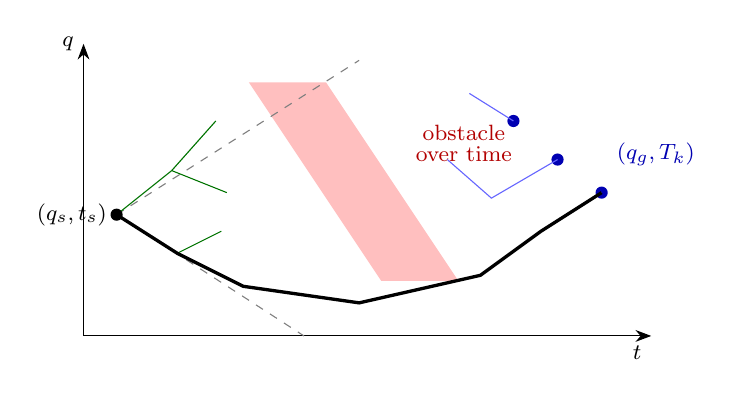
\begin{tikzpicture}[font=\footnotesize, x=7mm, y=7mm]
    \draw[-{Stealth[length=2mm]}] (0,0) -- (10.3,0) node[below left]{$t$};
    \draw[-{Stealth[length=2mm]}] (0,0) -- (0,5.3) node[left]{$q$};
    % moving obstacle in (q,t)
    \fill[red!25] (3.0,4.6) -- (4.4,4.6) -- (6.8,1.0) -- (5.4,1.0) -- cycle;
    \node[red!70!black, align=center] at (6.9,3.5) {obstacle\\[-2pt]over time};
    % reachable cone from start
    \draw[gray, dashed] (0.6,2.2) -- (5.0,5.0);
    \draw[gray, dashed] (0.6,2.2) -- (4.0,0.0);
    % goals
    \foreach \x/\y in {7.8/3.9, 8.6/3.2, 9.4/2.6} { \fill[blue!70!black] (\x,\y) circle (2.2pt); }
    \node[blue!70!black, right] at (9.5,3.3) {$(q_g, T_k)$};
    % start tree and goal tree
    \draw[thin, green!45!black] (0.6,2.2) -- (1.6,3.0) -- (2.4,3.9) (1.6,3.0) -- (2.6,2.6) (0.6,2.2) -- (1.7,1.5) -- (2.9,0.9) (1.7,1.5) -- (2.5,1.9);
    \draw[thin, blue!60] (7.8,3.9) -- (7.0,4.4) (8.6,3.2) -- (7.4,2.5) -- (6.6,3.2) (9.4,2.6) -- (8.3,1.9) -- (7.2,1.1);
    % solution path
    \draw[very thick, black] (0.6,2.2) -- (1.7,1.5) -- (2.9,0.9) -- (5.0,0.6) -- (7.2,1.1) -- (8.3,1.9) -- (9.4,2.6);
    \fill (0.6,2.2) circle (2.2pt) node[left]{$(q_s,t_s)$};
  \end{tikzpicture}
  \caption{Planning in space-time (schematic, one joint). A moving obstacle occupies a slanted region of
  $(q,t)$. The start tree (green) grows forward in time from the arm's future state; the goal tree
  (blue) grows backward from several timed pre-grasp goals. Edges may not exceed the joint velocity
  limits (dashed cone) and must move forward in time. The black path passes under the obstacle after it
  has gone.}
  \label{fig:spacetime}
\end{figure}

\textbf{Search.} An edge $(q_a,t_a)\to(q_b,t_b)$ is admissible if $t_b>t_a$, $|q_{b,j}-q_{a,j}| \le
v_{\max,j}(t_b-t_a)$ for every joint $j$, and the robot is collision-free along it with the world at the
matching times. As in ST-RRT*~\cite{grothe2022strrt}, samples are drawn only from the space-time
``double cone'' of states reachable from the start in time and from which some goal is still reachable.
Unlike ST-RRT*, the goal tree is rooted at \emph{many} goals (one per intercept time and arm posture), so
one search considers all of them, and the planner stops at the first connection. A shortcutting pass
replaces sub-paths with straight edges while keeping the knot times, so that the arrival time does not
change.

\textbf{Goals.} Intercept times span from 0.5\,s before the object becomes reachable until the tail no longer fits
in the episode. IK families are seeded with their own solution at the previous $T$, so each family is a
consistent arm posture. When a pre-grasp or tail collides, the planner searches the elbow's self-motion
(the one-dimensional null space of the gripper pose), since obstacles mostly meet the elbow rather than
the hand. Grasp candidates are top-down along both horizontal axes and tilted by $\pm35^\circ$.

\textbf{Executable motion.} Space-time plans cannot be retimed afterwards (for example by
TOPP-RA~\cite{pham2018toppra}), since their timing is what avoids the obstacles. The executed motion is a
$C^1$ cubic Hermite curve through the knots at their times. To keep its acceleration within per-joint
limits $a_{\max}$ (fractions of the reference limits used for the iiwa in~\cite{kiemel2024jerk}), every
knot must satisfy $|v_{\text{out}}-v_{\text{in}}|_j \le a_{\max,j}\min(h_{\text{in}},h_{\text{out}})/6$.
Extensions project their velocity into this window instead of rejecting samples, and the trees are joined
by exact single-edge shots that satisfy it at both ends. Before use, every plan is checked for joint
limits, 95\% of the velocity limits, the acceleration limits, joint torques by inverse dynamics (within
90\% of the datasheet), and collisions.

\textbf{Collision checking.} Signed-distance queries keep 3\,cm from obstacles and 5\,mm from the cart
and floor, sampling edges at least every 0.03\,rad and 0.04\,s. From the moment the gripper closes, the
held object moves with the gripper and must clear the obstacles too.

\textbf{Replanning and safety.} (B) replans every 0.5\,s from the state the arm will be in when planning
ends, keeping the executing trajectory as a prefix. Its budget is 0.25\,s (1.5\,s for the first plan),
and is raised when a collision is predicted. If the executing plan becomes unsafe, it tries cheap
\emph{escape primitives} (brake, go home, swing a joint, fold the arm), then a random-tree escape. After
the grasp, the arm must end somewhere it can stay safely, or the planner appends a gentle retreat with
the object in hand. \emph{Trade-off:} (B) is safe and executable by construction, but each plan takes
hundreds of milliseconds, and it only grasps when a goal is reachable within its limits.

\subsection{(C) Space-time trajectory optimization seeded by IK}

(C) plans the whole grasp as two problems in Drake's \texttt{KinematicTrajectoryOptimization} (full formulation: App.~\ref{app:C}): a clamped
cubic B-spline $q(s)=\sum_j b_j(s)P_j$ executed at $t=t_0+sT$. The \textbf{approach} problem is
\begin{equation}
\begin{aligned}
\min_{P,\,T}\ & T + 0.1\textstyle\sum_j \lVert P_{j+1}-P_j\rVert^2\\
\text{s.t.}\ & q(0)=q_0,\ \dot q(0)=v_0,\ |\ddot q|\le 4\,\text{rad/s}^2,\\
& \text{joint and velocity limits},\\
& \text{grasp pose of time } t_0+T \text{ at } s=1, \text{ moving with it},\\
& \text{hover 10\,cm above it at } s_d, \text{ straight descent},\\
& d_O(q(s_k), t_0+s_kT)\ge 4\,\text{cm},\ d_{\text{env}}\ge 5\,\text{mm},\\
& s_k = k/30,\ k=1,\dots,30,
\end{aligned}
\label{eq:kto}
\end{equation}
where $d_O$ is the minimum signed distance to the obstacles posed where they will be at that time. The
duration $T$ is free, so the world's configuration enters the constraints as a function of $T$ and its
gradient includes the obstacles' motion. A second \textbf{hold} problem, of fixed duration to the end of
the scene, closes the gripper while moving with the object, lifts it 10\,cm and keeps clear of the
obstacles.

\textbf{Seeding.} Collision-aware IK finds a grasp and hover pose at candidate grasp times, starting
from when the object passes closest to the robot, plus the earliest feasible one. Initial guesses are
straight joint-space lines to these poses, the same through collision-free halfway configurations, and
lines to later grasp times. Four worker processes solve the guesses in parallel with SNOPT at a loose
tolerance, then refine them while time remains, and (C) keeps the lowest-cost plan.

\textbf{Timing.} Planning starts 2\,s before $t_0$ and the arm holds still meanwhile. A plan that arrives
late is rejected and redone with 1.5$\times$ the time it took. Without a plan, (C) replans at every update
until 1.2\,s before the object leaves reach. If an obstacle would hit the parked arm first, a small \emph{dodge}
optimization moves it out of the way. \emph{Trade-off:} (C) finds the fastest grasps, but solve times are
unbounded, so a plan, or even a dodge, can arrive too late.

\subsection{(D) Learned policy: BC $\to$ DAgger $\to$ PPO}

\textbf{Policy.} A $3\times512$ ReLU MLP runs every 0.1\,s (full formulation: App.~\ref{app:D}). Its 84 inputs are the exact state: joint
positions and commanded velocities, gripper opening and pose, the grasp-pose error in the gripper frame,
the object's velocity and width, the four nearest obstacles (relative position, velocity, half extents,
distance to the robot, presence flag), and the times until the object enters and leaves reach. It outputs
the means of eight Gaussian actions: seven joint target velocities (through $\tanh$, reached by an
acceleration-limited ramp) and the gripper width, with learned, state-independent noise.

\textbf{Training.} Training uses a mix of fresh scenes (60\% like the held-out generator, 40\% blockers)
that never includes a test scene.
\begin{enumerate}
  \item \emph{Behavior cloning} on 34{,}981 successful episodes of (C) (4.4M state-action pairs), with
    small state noise.
  \item \emph{DAgger}~\cite{ross2011dagger}: after some policy episodes, the policy's actions are replayed
    up to a random time before failure, (C) plans from the moving robot with the simulation paused, and,
    if (C) succeeds, its actions become labels (5.0M in all).
  \item \emph{PPO}~\cite{schulman2017ppo} with GAE ($\gamma=0.99$, $\lambda=0.95$)~\cite{schulman2016gae},
    in its decoupled form for asynchronous workers~\cite{hilton2022batch}, with an imitation loss on
    (C)'s demonstrations and DAgger labels whose weight is ramped down as the PPO weight ramps up.
\end{enumerate}
The reward combines potential-based shaping terms~\cite{ng1999shaping} for progress toward the grasp pose
and for clearance from obstacles, the cart and the floor, a bonus for closing at the grasp pose at the
object's velocity, and terminal rewards ($+1$ success, $-1$ collision or drop, $-2$ for a failure after
success). Training runs on about 400 CPU workers feeding one GPU learner, and the selected checkpoint
(42.7M steps, 3.9\,h) is the best on 500 new scenes from the training mix, never trained on (Train-500). Table~\ref{tab:rl} in the
appendix lists the full schedule and hyperparameters. \emph{Trade-off:} (D) decides in about a
millisecond, but it has no collision guarantee and depends on its training distribution.

% ---------------------------------------------------------------------------------------------------
\section{Experimental Setup}
\label{sec:setup}

\textbf{Scene sets.} We evaluate on 214 fixed scenes:
\begin{itemize}
  \item \emph{dev} (20): generated scenes used during development;
  \item \emph{preset grids} (114): a 0.4\,m post (48) or a thin plank (48) that crosses the straight line
    from the base to the object exactly when a direct grasp would happen, gridded over target speed,
    obstacle speed and crossing time, and a 1.6\,m pillar that can only be passed on one side, combined with a
    faster post (18);
  \item \emph{held-out} (80): generated from a separate seed and not used for tuning, although some of its
    failures were inspected during development.
\end{itemize}

\textbf{Protocol.} All runs use measured latency (Section~\ref{sec:problem}) on 10-core Apple-silicon
laptops, with eight episodes in parallel; every non-success is then rerun alone and that result counts,
so that contention between parallel episodes does not cause failures. Each controller is evaluated once
per scene at a fixed commit of the shared repository. Because measured latency is wall time, results vary
slightly between runs: for (B), repeated runs of the held-out set differ by about $\pm2$ scenes.

\textbf{Metrics.} Each metric maps to a design goal: success and the failure mode (G1, G2); time from
the object entering reach to the grasp (G1); minimum obstacle clearance (G2); peak commanded joint speed
and peak joint torque from inverse dynamics, as fractions of the limits (G3); and compute per plan or per
decision, including failed attempts (G4).

% ---------------------------------------------------------------------------------------------------
\section{Results and Discussion}
\label{sec:results}

\begin{table}[t]
  \centering
  \caption{Successes per scene set (measured latency, scored to the end of each scene). Bold: best.}
  \label{tab:success}
  \setlength{\tabcolsep}{3pt}\small
  \begin{tabular}{@{}lccccc@{}}
    \toprule
    & dev & grids & held-out & all & coll./t.o./drop \\
    & (20) & (114) & (80) & (214) & \\
    \midrule
    Naive$^\dagger$ & -- & -- & 35 & -- & 40 collisions \\
    (A) reactive QP     & 11 & 69  & 52 & 132 & 6 / 71 / 5 \\
    (B) ST-RRT  & 15 & 95  & 63 & 173 & \textbf{0} / 41 / \textbf{0} \\
    (C) traj.\ opt. & 17 & 106 & \textbf{72} & \textbf{195} & 9 / 10 / \textbf{0} \\
    \midrule
    (D) BC              & 10 & 104 & 37 & 151 & 58 / 2 / 3 \\
    (D) BC + DAgger     & 11 & 106 & 38 & 155 & 57 / 2 / \textbf{0} \\
    (D) PPO             & \textbf{18} & \textbf{113} & 62 & 193 & 17 / 1 / 3 \\
    \bottomrule
  \end{tabular}\\[2pt]
  {\footnotesize $^\dagger$No obstacle avoidance; held-out set only, counted at the first success, before end-of-scene scoring.}
\end{table}

\begin{table}[t]
  \centering
  \caption{Quality of the motion over all 214 scenes (medians over episodes).}
  \label{tab:quality}
  \setlength{\tabcolsep}{3.5pt}
  \begin{tabular}{@{}lcccc@{}}
    \toprule
    & (A) & (B) & (C) & (D) PPO \\
    \midrule
    Time to grasp after object in reach (s)  & 2.21 & 2.66 & 1.60 & \textbf{1.24} \\
    Min.\ obstacle clearance (cm)            & 5.3  & \textbf{5.5} & 4.1 & 3.3 \\
    Peak torque (fraction of limit)          & 2.20 & \textbf{0.34} & 0.44 & 0.47 \\
    Peak joint speed (fraction of limit)     & 0.60 & \textbf{0.44} & 0.59 & 0.49 \\
    Compute per plan / decision (ms)         & 2.2  & 862  & 1492 & \textbf{1.24} \\
    \bottomrule
  \end{tabular}
\end{table}

\begin{figure}[t]
  \centering
  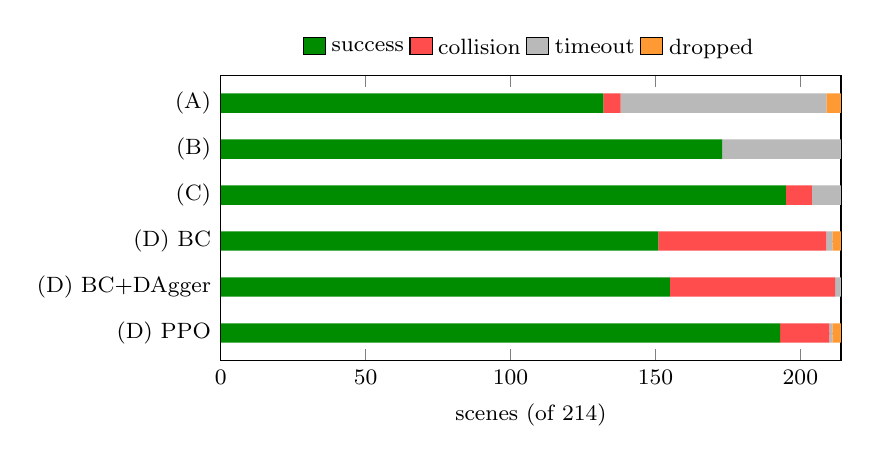
\begin{tikzpicture}
    \begin{axis}[
        xbar stacked, width=0.78\columnwidth, height=5.2cm, bar width=7pt,
        xmin=0, xmax=214, xlabel={scenes (of 214)},
        ytick={1,...,6}, yticklabels={(D) PPO,(D) BC+DAgger,(D) BC,(C),(B),(A)},
        legend style={at={(0.5,1.02)}, anchor=south, legend columns=4, font=\footnotesize, draw=none},
        tick label style={font=\footnotesize}, label style={font=\footnotesize}, enlarge y limits=0.12]
      \addplot[fill=green!55!black, draw=none] coordinates {(132,6) (173,5) (195,4) (151,3) (155,2) (193,1)};
      \addplot[fill=red!70, draw=none] coordinates {(6,6) (0,5) (9,4) (58,3) (57,2) (17,1)};
      \addplot[fill=gray!55, draw=none] coordinates {(71,6) (41,5) (10,4) (2,3) (2,2) (1,1)};
      \addplot[fill=orange!80, draw=none] coordinates {(5,6) (0,5) (0,4) (3,3) (0,2) (3,1)};
      \legend{success, collision, timeout, dropped}
    \end{axis}
  \end{tikzpicture}
  \caption{Outcomes on all 214 scenes. The planners differ mainly in how they fail: (A) and (B) time out
  when they cannot get past an obstacle, while the learned policy almost never times out but collides
  more often.}
  \label{fig:outcomes}
\end{figure}

Table~\ref{tab:success} and Fig.~\ref{fig:outcomes} summarize the outcomes, and
Table~\ref{tab:quality} the quality of the motion.

\textbf{Safety vs.\ success.} (B) is the only method with no collisions and no drops in all 214 scenes
(G2), and its motion stays at 34\% of the torque limits (G3). Its 41 failures are all timeouts: it
abstains rather than risk a collision. (C) grasps the most (195) and fastest (median 1.60\,s after the
object comes into reach), with lower clearance (4.1\,cm) and 9 collisions. (A) times out in 71 scenes,
mostly behind obstacles that must be gone around: it grasps 2 of the 18 pillar scenes, against 6 for (B)
and 10 for (C). Its velocity steps between phases also exceed the torque limits (median peak 2.2$\times$),
so (A) fails G3 even when it succeeds.

\textbf{Are (B)'s abstentions correct?} To tell whether (B) missed grasps that were possible, we certified
each held-out scene it did not grasp. An exhaustive goal search (dense intercept times, many IK seeds and
elbow postures, (B)'s grasp candidates and grasp tail) tests whether any goal exists; an \emph{oracle},
the same planner with 20$\times$ the compute and planning time free, tests whether a plan to one exists;
and repeating the oracle at higher acceleration limits gives the acceleration each scene needs.
Table~\ref{tab:cert} shows the result. In 7 scenes no goal exists at all, and in 6 more goals exist but
even the oracle finds no plan within (B)'s limits (two of these become possible at $1.33\times$ its
acceleration). So at most 67 of the 80 held-out scenes can be solved within (B)'s grasp model and limits,
and (B) grasps 63. The remaining 4 are solved by the oracle at (B)'s own limits: there, the online
planner's compute budget, not the problem, is what fails, which is the case for faster collision checking
made in Section~\ref{sec:conclusion}. The verdicts are relative to (B)'s goals, not absolute: (C), with its
own grasp poses and seeding, grasps 9 of the 17 scenes, including one with no goal for (B)
(\texttt{mix\_0028}) and three where (B)'s oracle fails. (B)'s gap to (C) on the held-out set (63 vs.\ 72)
is therefore mostly goal coverage, and partly compute. (D) PPO grasps 5 of the 17; in all 7 scenes with no goal for (B), it collides instead of abstaining.

\begin{table}[t]
  \centering
  \caption{Certification of the 17 held-out scenes (B) does not grasp, and how many of them (C) and (D) PPO grasp.}
  \label{tab:cert}
  \setlength{\tabcolsep}{4pt}
  \begin{tabular}{@{}lccc@{}}
    \toprule
    Verdict for (B) & scenes & \multicolumn{2}{c}{grasps} \\
    \cmidrule(l){3-4}
    & & (C) & (D) \\
    \midrule
    No goal in (B)'s grasp model                        & 7 & 1 & 0 \\
    Goals exist, no plan even for the oracle$^\ast$      & 6 & 4 & 3 \\
    Oracle succeeds at (B)'s limits (missed online)     & 4 & 4 & 2 \\
    \midrule
    Total                                               & 17 & 9 & 5 \\
    \bottomrule
  \end{tabular}\\[2pt]
  {\footnotesize $^\ast$Two become possible at $1.33\times$ (B)'s acceleration limits.}
\end{table}

\textbf{Compute.} (B) needs 862\,ms and (C) 1.5\,s per plan, while (A) and (D) decide in about a
millisecond (G4). (D) is this fast because it moves the computation to training: (C)'s demonstrations and DAgger
labels, then 3.9\,h of PPO on about 400 CPU cores and one GPU. Because compute costs time, slow plans fail in a specific way: 7 of (C)'s 9 collisions
are pillar scenes where the dodge takes 1.4--20\,s to compute, and in the other two the arm is hit while
parked as a late first plan arrives. The policy (D) avoids this entirely: it recovers 193 of (C)'s 195
successes at about 1/1200 of its compute.

\textbf{Learning.} BC alone reaches 151 successes, but with 58 collisions, the classic symptom of
compounding errors away from the expert's states. DAgger barely helps (155), while PPO fine-tuning cuts
collisions from 58 to 17 and raises Train-500 success from 66\% to 90\%. The policy is best on the preset
grids (113 of 114), which resemble its training blockers, but falls behind (B) and (C) on the held-out
set (62), where 15 of its 18 failures are collisions: it generalizes less well to unseen obstacle
configurations than the planners, which check every motion against the predicted obstacles.

\textbf{Examples.} Fig.~\ref{fig:examples} shows held-out scenes in which the methods differ, and
Fig.~\ref{fig:ppo} a scene in which only the policy succeeds. Together they illustrate the failure modes
above: drops caused by (A)'s abrupt motion, (B) waiting in an escape pose, and (C)'s late plans.

\begin{figure*}[t]
  \centering
  \setlength{\tabcolsep}{1pt}
  \begin{tabular}{@{}cccc@{}}
    scene, $t=0$ & (A) reactive & (B) space-time RRT & (C) trajectory opt. \\
    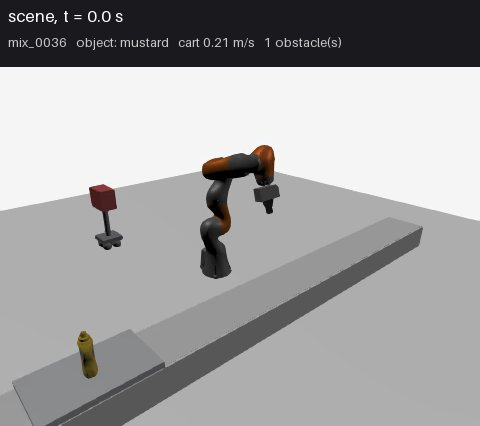
\includegraphics[width=0.24\textwidth]{frames/mix_0036_0.jpg} &
    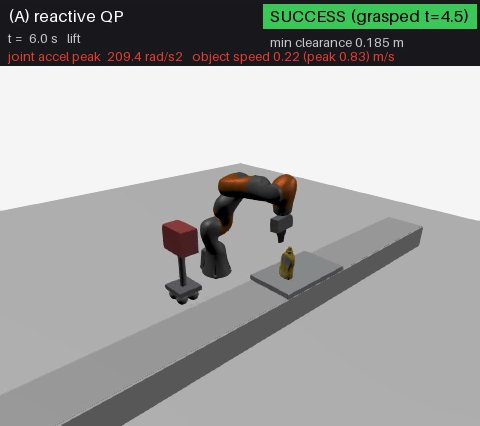
\includegraphics[width=0.24\textwidth]{frames/mix_0036_1.jpg} &
    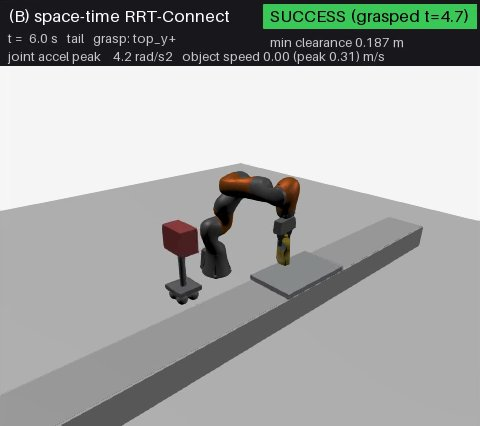
\includegraphics[width=0.24\textwidth]{frames/mix_0036_2.jpg} &
    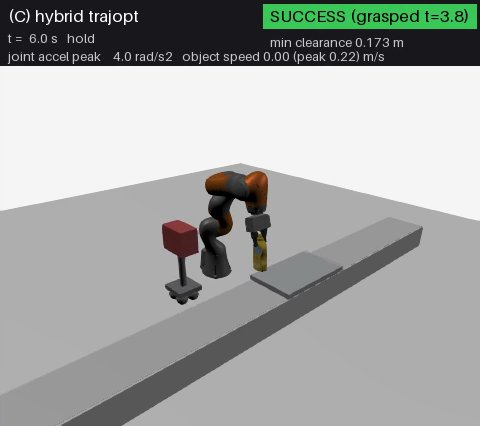
\includegraphics[width=0.24\textwidth]{frames/mix_0036_3.jpg} \\
    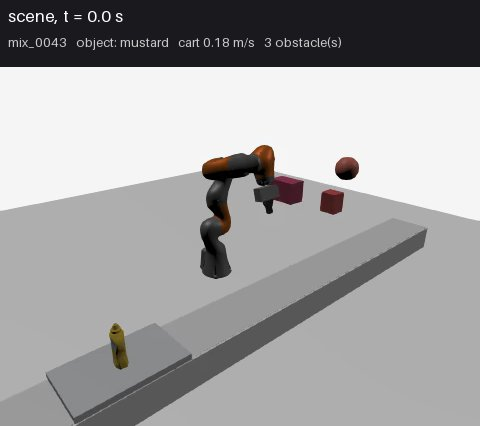
\includegraphics[width=0.24\textwidth]{frames/mix_0043_0.jpg} &
    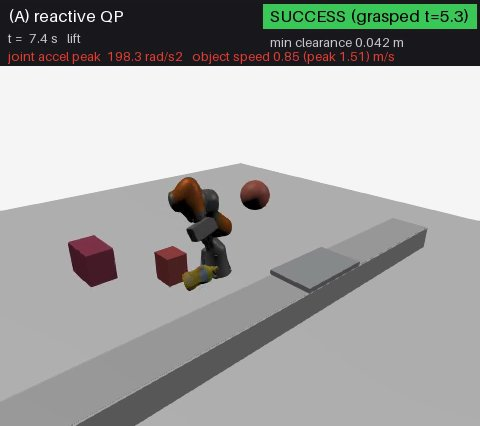
\includegraphics[width=0.24\textwidth]{frames/mix_0043_1.jpg} &
    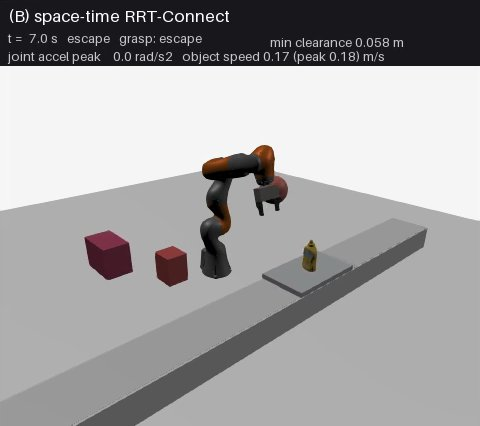
\includegraphics[width=0.24\textwidth]{frames/mix_0043_2.jpg} &
    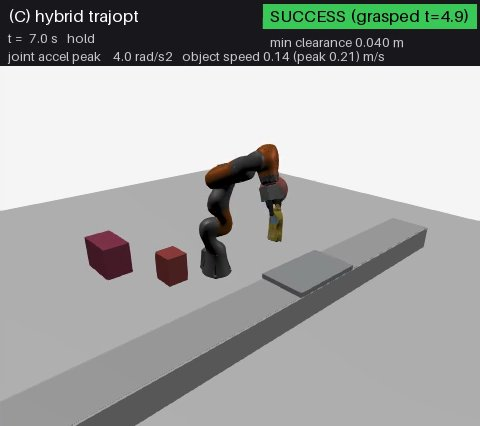
\includegraphics[width=0.24\textwidth]{frames/mix_0043_3.jpg} \\
    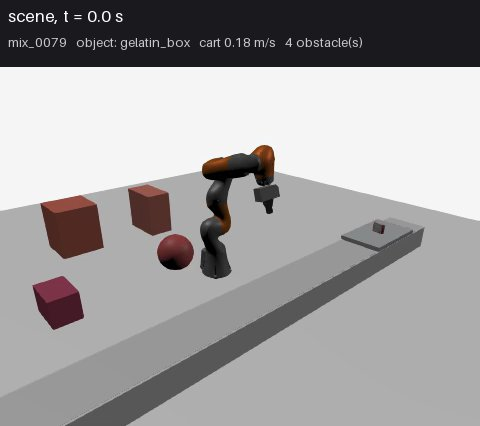
\includegraphics[width=0.24\textwidth]{frames/mix_0079_0.jpg} &
    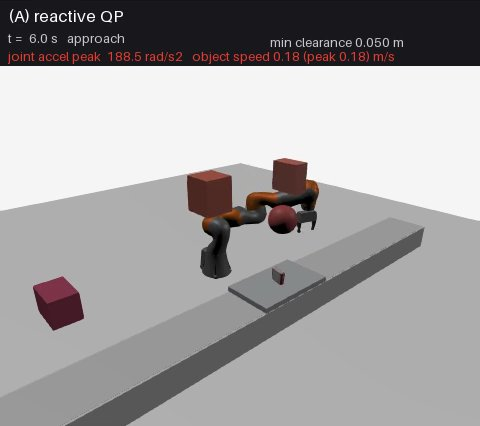
\includegraphics[width=0.24\textwidth]{frames/mix_0079_1.jpg} &
    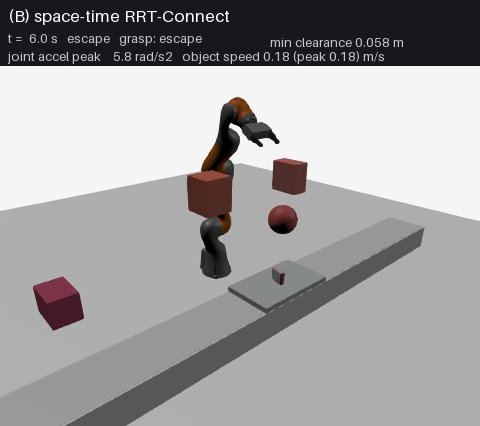
\includegraphics[width=0.24\textwidth]{frames/mix_0079_2.jpg} &
    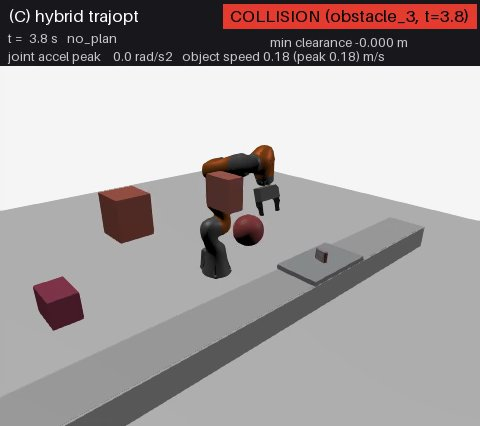
\includegraphics[width=0.24\textwidth]{frames/mix_0079_3.jpg} \\
  \end{tabular}
  \caption{Held-out examples. \emph{Top} (\texttt{mix\_0036}, \vid{mix_0036}): all three grasp the mustard
  bottle, but it slips out of (A)'s gripper right after the lift. \emph{Middle} (\texttt{mix\_0043},
  \vid{mix_0043}): two boxes and a sphere pass the arm; (A) grasps late and flings the bottle away while
  swerving around the sphere, (B) never leaves its escape pose, and only (C) holds the object.
  \emph{Bottom} (\texttt{mix\_0079}, \vid{mix_0079}): three boxes and a sphere crowd the arm; (A) cannot
  get past them, (B) escapes and times out, and (C)'s plan arrives too late, so a box hits the parked arm.
  This scene is one of the six that even (B)'s oracle cannot solve.}
  \label{fig:examples}
\end{figure*}

\begin{figure}[t]
  \centering
  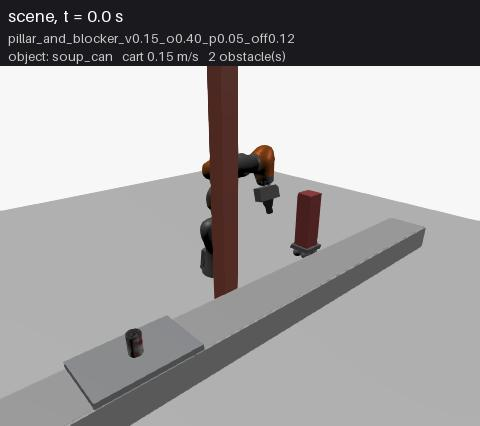
\includegraphics[width=0.325\columnwidth]{frames/pillar_and_blocker_v0.15_o0.40_p0.05_off0.12_0.jpg}\hfill
  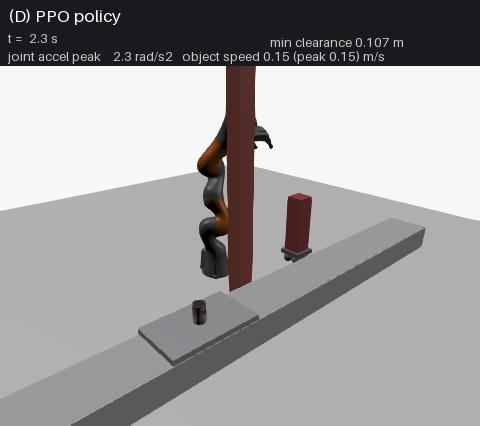
\includegraphics[width=0.325\columnwidth]{frames/pillar_and_blocker_v0.15_o0.40_p0.05_off0.12_1.jpg}\hfill
  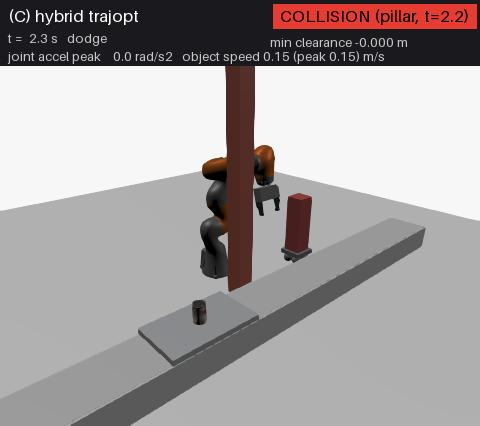
\includegraphics[width=0.325\columnwidth]{frames/pillar_and_blocker_v0.15_o0.40_p0.05_off0.12_2.jpg}
  \caption{A pillar sweeps through the start pose (left, $t=0$). The policy (D, middle) pulls the arm
  back and grasps at 5.7\,s; (C, right) is still computing its dodge when the pillar hits it at 2.2\,s
  (frames at 2.3\,s; \vid{pillar_and_blocker_v0.15_o0.40_p0.05_off0.12}).}
  \label{fig:ppo}
\end{figure}

\textbf{Back to the design goals.} No method meets all four goals. (B) is the only one that meets G2 and
G3 throughout, at the cost of G1 and G4. (C) comes closest to G1 but violates G2 when its computation
runs late. (D) meets G4 and nearly matches (C) on G1, but not G2 on unseen scenes. (A) meets G4 only.
This suggests combining the methods: a fast policy or reactive layer for real-time response, with a
planner's collision check as a safety filter, or a planner warm-started by the policy.

% ---------------------------------------------------------------------------------------------------
\section{Limitations and Conclusion}
\label{sec:conclusion}

\textbf{Limitations.}
(i) \emph{Exact prediction.} Every controller is given the true future motion of the scene. With perfect
prediction, a valid plan never goes stale, which favors the deliberative methods.
(ii) \emph{No perception.} The object's pose, identity and geometry are known.
(iii) \emph{Simulation only}, with a rigid model of the held object (no slip in (B)'s checks).
(iv) \emph{Goal coverage.} 13 of (B)'s 17 held-out misses have no goal or no plan in its grasp model;
more grasp types and a shorter grasp tail at high cart speeds would help.
(v) \emph{Compute.} (B) spends about 70\,$\mu$s per state check, and 4 of its held-out misses are
solvable with more compute; a vectorized checker such as VAMP~\cite{thomason2024vamp} would allow more
replans and larger trees.
(vi) \emph{Evaluation.} Measured latency depends on the machine, and some held-out failures were inspected
during development.

\textbf{Conclusion.} We compared four ways to grasp a moving object among moving obstacles on a shared
benchmark that charges computation against the clock and scores to the end of the scene. Deliberative
space-time planning gives the safest, most executable motion, trajectory optimization reaches the most
grasps, and a policy distilled from the optimizer and fine-tuned with PPO recovers nearly all of its
successes at a millisecond per decision, but collides more in scenes unlike its training data.

\textbf{Next: perception.} Our next step is to remove the most unrealistic assumption, that the scene is
known exactly. The simulated station already has cameras; we plan to estimate the object's pose from
point clouds \todo{method: e.g.\ geometric registration against the known model, or a learned grasp
detector~\cite{sundermeyer2021contactgraspnet,zhai2023monograspnet}}, track the obstacles and predict their
motion from noisy observations, and measure how each controller degrades as prediction error grows.
Replanning methods such as (B) should then gain on methods that commit to one plan.
\todo{scope of the perception extension and who owns it.}

% ---------------------------------------------------------------------------------------------------
\section*{Acknowledgments}

We thank the 6.4212 course staff, in particular Guillermo Mendoza Contreras, for feedback on the project
scope. \textbf{AI use.} Implementations of the experiments used AI after the initial experiments were designed and the scenes were implemented. Additionally, Claude and ChatGPT were used to help structure this report before being revised by the authors.

\begin{thebibliography}{99}

\bibitem{allen1993tracking}
P.~K. Allen, A.~Timcenko, B.~Yoshimi, and P.~Michelman, ``Automated tracking and grasping of a moving
object with a robotic hand-eye system,'' \emph{IEEE Trans. Robot. Autom.}, vol.~9, no.~2, pp.~152--165,
1993.

\bibitem{marturi2019dynamic}
N.~Marturi, M.~Kopicki, A.~Rastegarpanah, V.~Rajasekaran, M.~Adjigble, R.~Stolkin, A.~Leonardis, and
Y.~Bekiroglu, ``Dynamic grasp and trajectory planning for moving objects,'' \emph{Auton. Robots},
vol.~43, no.~5, pp.~1241--1256, 2019.

\bibitem{akinola2021dynamic}
I.~Akinola, J.~Xu, S.~Song, and P.~K. Allen, ``Dynamic grasping with reachability and motion
awareness,'' in \emph{Proc. IEEE/RSJ Int. Conf. Intell. Robots Syst. (IROS)}, 2021.

\bibitem{fiorini1998velocity}
P.~Fiorini and Z.~Shiller, ``Motion planning in dynamic environments using velocity obstacles,''
\emph{Int. J. Robot. Res.}, vol.~17, no.~7, pp.~760--772, 1998.

\bibitem{kuffner2000rrtconnect}
J.~J. Kuffner and S.~M. LaValle, ``RRT-Connect: An efficient approach to single-query path planning,'' in
\emph{Proc. IEEE Int. Conf. Robot. Autom. (ICRA)}, 2000.

\bibitem{grothe2022strrt}
F.~Grothe, V.~N. Hartmann, A.~Orthey, and M.~Toussaint, ``ST-RRT*: Asymptotically-optimal bidirectional
motion planning through space-time,'' in \emph{Proc. IEEE Int. Conf. Robot. Autom. (ICRA)}, 2022.

\bibitem{thomason2024vamp}
W.~Thomason, Z.~Kingston, and L.~E. Kavraki, ``Motions in microseconds via vectorized sampling-based
planning,'' in \emph{Proc. IEEE Int. Conf. Robot. Autom. (ICRA)}, 2024.

\bibitem{khatib1986realtime}
O.~Khatib, ``Real-time obstacle avoidance for manipulators and mobile robots,'' \emph{Int. J. Robot.
Res.}, vol.~5, no.~1, pp.~90--98, 1986.

\bibitem{faverjon1987local}
B.~Faverjon and P.~Tournassoud, ``A local based approach for path planning of manipulators with a high
number of degrees of freedom,'' in \emph{Proc. IEEE Int. Conf. Robot. Autom. (ICRA)}, 1987.

\bibitem{haviland2021neo}
J.~Haviland and P.~Corke, ``NEO: A novel expeditious optimisation algorithm for reactive motion control
of manipulators,'' \emph{IEEE Robot. Autom. Lett.}, vol.~6, no.~2, pp.~1043--1050, 2021.

\bibitem{ratliff2009chomp}
N.~Ratliff, M.~Zucker, J.~A. Bagnell, and S.~Srinivasa, ``CHOMP: Gradient optimization techniques for
efficient motion planning,'' in \emph{Proc. IEEE Int. Conf. Robot. Autom. (ICRA)}, 2009.

\bibitem{schulman2014trajopt}
J.~Schulman, Y.~Duan, J.~Ho, A.~Lee, I.~Awwal, H.~Bradlow, J.~Pan, S.~Patil, K.~Goldberg, and
P.~Abbeel, ``Motion planning with sequential convex optimization and convex collision checking,''
\emph{Int. J. Robot. Res.}, vol.~33, no.~9, pp.~1251--1270, 2014.

\bibitem{tedrake2019drake}
R.~Tedrake and the Drake Development Team, ``Drake: Model-based design and verification for robotics,''
2019. [Online]. Available: https://drake.mit.edu

\bibitem{tedrake2024manipulation}
R.~Tedrake, \emph{Robotic Manipulation: Perception, Planning, and Control}, course notes for MIT 6.4210.
[Online]. Available: http://manipulation.mit.edu

\bibitem{gill2005snopt}
P.~E. Gill, W.~Murray, and M.~A. Saunders, ``SNOPT: An SQP algorithm for large-scale constrained
optimization,'' \emph{SIAM Rev.}, vol.~47, no.~1, pp.~99--131, 2005.

\bibitem{stellato2020osqp}
B.~Stellato, G.~Banjac, P.~Goulart, A.~Bemporad, and S.~Boyd, ``OSQP: An operator splitting solver for
quadratic programs,'' \emph{Math. Program. Comput.}, vol.~12, no.~4, pp.~637--672, 2020.

\bibitem{pham2018toppra}
H.~Pham and Q.-C. Pham, ``A new approach to time-optimal path parameterization based on reachability
analysis,'' \emph{IEEE Trans. Robot.}, vol.~34, no.~3, pp.~645--659, 2018.

\bibitem{kiemel2024jerk}
J.~C. Kiemel and T.~Kr\"oger, ``Jerk-limited traversal of one-dimensional paths and its application to
multi-dimensional path tracking,'' in \emph{Proc. IEEE Int. Conf. Robot. Autom. (ICRA)}, 2024,
arXiv:2407.13423.

\bibitem{fishman2022mpinets}
A.~Fishman, A.~Murali, C.~Eppner, B.~Peele, B.~Boots, and D.~Fox, ``Motion policy networks,'' in
\emph{Proc. Conf. Robot Learn. (CoRL)}, 2022.

\bibitem{ross2011dagger}
S.~Ross, G.~J. Gordon, and J.~A. Bagnell, ``A reduction of imitation learning and structured prediction
to no-regret online learning,'' in \emph{Proc. Int. Conf. Artif. Intell. Statist. (AISTATS)}, 2011.

\bibitem{schulman2017ppo}
J.~Schulman, F.~Wolski, P.~Dhariwal, A.~Radford, and O.~Klimov, ``Proximal policy optimization
algorithms,'' arXiv:1707.06347, 2017.

\bibitem{schulman2016gae}
J.~Schulman, P.~Moritz, S.~Levine, M.~Jordan, and P.~Abbeel, ``High-dimensional continuous control using
generalized advantage estimation,'' in \emph{Proc. Int. Conf. Learn. Represent. (ICLR)}, 2016.

\bibitem{hilton2022batch}
J.~Hilton, K.~Cobbe, and J.~Schulman, ``Batch size-invariance for policy optimization,'' in \emph{Adv.
Neural Inf. Process. Syst. (NeurIPS)}, 2022.

\bibitem{ng1999shaping}
A.~Y. Ng, D.~Harada, and S.~Russell, ``Policy invariance under reward transformations: Theory and
application to reward shaping,'' in \emph{Proc. Int. Conf. Mach. Learn. (ICML)}, 1999.

\bibitem{calli2015ycb}
B.~Calli, A.~Walsman, A.~Singh, S.~Srinivasa, P.~Abbeel, and A.~M. Dollar, ``Benchmarking in
manipulation research: Using the Yale-CMU-Berkeley object and model set,'' \emph{IEEE Robot. Autom.
Mag.}, vol.~22, no.~3, pp.~36--52, 2015.

\bibitem{sundermeyer2021contactgraspnet}
M.~Sundermeyer, A.~Mousavian, R.~Triebel, and D.~Fox, ``Contact-GraspNet: Efficient 6-DoF grasp
generation in cluttered scenes,'' in \emph{Proc. IEEE Int. Conf. Robot. Autom. (ICRA)}, 2021.

\bibitem{zhai2023monograspnet}
G.~Zhai, D.~Huang, S.-C. Wu, H.~Jung, Y.~Di, F.~Manhardt, F.~Tombari, N.~Navab, and B.~Busam,
``MonoGraspNet: 6-DoF grasping with a single RGB image,'' in \emph{Proc. IEEE Int. Conf. Robot. Autom.
(ICRA)}, 2023.

\end{thebibliography}

% ---------------------------------------------------------------------------------------------------
\appendices
\section{Method details}
\label{app:methods}

Values are those of the 214-scene evaluation, which builds every controller with its defaults.

\emph{Notation.} \emph{Robot:} $q,\dot q,\ddot q$: joint positions, velocities, accelerations; $q_{lo},q_{hi}$,
$v_{\max}$: joint limits and speed limits (datasheet); $a_{\text{ref}}=(15,7.5,10,12.5,15,20,20)$\,rad/s$^2$:
reference joint accelerations~\cite{kiemel2024jerk}; $X_G=(R_G,p_G)$: pose of the WSG body, $\omega_G,v_G$: its
angular and linear velocity, $J(q)\in\mathbb R^{6\times7}$: its [angular; linear] Jacobian; opening 0.107\,m
(open) to 0 (closed). \emph{Scene:} $X^*(t)=(R^*,p^*(t))$: the gripper pose that grasps the object at time $t$
(top-down; (B) also tries others); $v_{\text{obj}}$: the object's velocity (the cart's); $\hat z$: up; $z_G$, $z^*$:
heights of $p_G$, $p^*$; $t_{\text{enter}},t_{\text{exit}}$: when the object enters and leaves reach; $t_{\text{end}}$:
end of the scene. \emph{Geometry:} the robot is links 1--7, the WSG body and its open fingers; $\phi$: a signed
distance between it and the world posed as predicted at the queried time; $d$: a required clearance. Gripper--object
contact never counts, since a grasp is such contact. \emph{Motion:} $x\in[0,1]$: progress through a timed motion;
$m(x)=10x^3-15x^4+6x^5$: minimum-jerk profile (0 to 1, zero velocity and acceleration at both ends); $\tau$: time
since a motion's start. Vector inequalities and $|\cdot|$ hold per component.

% ---------------------------------------------------------------------------------------------------
\subsection{(A) Reactive QP}
\label{app:A}

Every 10\,ms, at the measured $q$ and $X_G$, (A) finds the joint velocities that best track a target twist while no
robot--world pair closes faster than its distance allows:
\begin{equation}
\begin{aligned}
\min_{\dot q,\,s}\ & \lVert W(J\dot q-V)\rVert^2+\lambda\lVert\dot q\rVert^2+\mu\lVert\dot q-\dot q_{\text{prev}}\rVert^2\\
& +100\textstyle\sum_i s_i+1000\lVert s\rVert^2\\
\text{s.t.}\ & n_i^\top J_{r,i}\,\dot q+s_i\ \ge\ -\xi(\phi_i-d_i)+n_i^\top v_{w,i},\quad s_i\ge0,\\
& \tfrac{q_{lo}+0.05-q}{0.2}\le\dot q\le\tfrac{q_{hi}-0.05-q}{0.2},\quad|\dot q|\le0.6\,v_{\max}.
\end{aligned}
\label{eq:qpfull}
\end{equation}
\begin{itemize}
  \item \emph{Target twist:} $V=\big[k_R\,e_R;\ \operatorname{sat}(k_p e_p+v_{\text{ff}})\big]$, a pull towards the
    phase's target pose $(R_d,p_d)$ plus a feedforward velocity $v_{\text{ff}}$ (Table~\ref{tab:phasesA});
    $e_R$: axis-angle of $R_dR_G^\top$, $e_p=p_d-p_G$; $k_R=k_p=4\,\text{s}^{-1}$;
    $\operatorname{sat}(v)=v\min(1,0.8/\lVert v\rVert)$ caps the linear part at 0.8\,m/s (the angular part is not
    capped).
  \item \emph{Dampers}, one row per pair $i$ closer than 25\,cm between the robot at $q$ and the world (obstacles,
    cart, floor, object) as predicted at $t$, $t+0.1$ and $t+0.2$\,s; gripper--object pairs are left out so that the
    gripper can grasp. $\phi_i$: signed distance; $n_i$: unit normal from the world to the robot witness point;
    $J_{r,i}$: translational Jacobian of the robot witness point; $v_{w,i}$: predicted velocity of the world
    witness point; $d_i$: 4\,cm (obstacles), 5\,mm (cart, floor, object); $\xi=2\,\text{s}^{-1}$. As
    $\dot\phi_i=n_i^\top(J_{r,i}\dot q-v_{w,i})$, with $s_i=0$ the row is $\dot\phi_i\ge-\xi(\phi_i-d_i)$: the pair
    may close at most at rate $\xi(\phi_i-d_i)$, so $\phi_i$ falls towards $d_i$ no faster than exponentially. The
    slacks $s$ keep the QP feasible when dampers conflict.
  \item \emph{Joint limits:} each joint may approach its limit (minus 0.05\,rad) at most fast enough to reach it in
    0.2\,s; speeds stay within $0.6\,v_{\max}$.
  \item \emph{Weights:} $W=I_6$, and $\operatorname{diag}(1,1,1,1,1,10)$ in the lift (the height error counts
    100$\times$); $\lambda=\mu=5\cdot10^{-3}$; $\dot q_{\text{prev}}$: the last cycle's $\dot q$.
  \item \emph{Solve and command:} OSQP on a Drake program built every cycle ($\dot q=0$ if it fails);
    $q_{\text{cmd}}\leftarrow\operatorname{clip}(q_{\text{cmd}}+0.01\,\dot q,\ q_{lo},q_{hi})$.
  \item \emph{Lift reference:} over 0.6\,s from the lift's start $t_L$, the gripper's horizontal velocity decays from
    the object's to 0 along $1-m(x)$ while its height rises 10\,cm along $m(x)$; then it holds. With
    $x=\operatorname{clip}\big((t-t_L)/0.6,0,1\big)$, $p_0=p_G(t_L)$ and $v_h$ the horizontal part of
    $v_{\text{obj}}(t_L)$: $\dot p_L=(1-m(x))\,v_h+\tfrac{0.1}{0.6}m'(x)\hat z$, and its integral
    $p_L=p_0+0.6\,v_h(x-2.5x^4+3x^5-x^6)+0.1\,m(x)\hat z$.
\end{itemize}

\begin{table}[!t]
  \centering
  \caption{Phases of (A).}
  \label{tab:phasesA}
  \footnotesize\setlength{\tabcolsep}{2.5pt}
  \begin{tabular}{@{}lllc>{\raggedright\arraybackslash}p{0.3\columnwidth}@{}}
    \toprule
    phase & target $(R_d,p_d)$ & $v_{\text{ff}}$ & gripper & next phase when \\
    \midrule
    wait     & $X_G$ at $t=0$             & 0                 & open   & $t\ge t_{\text{enter}}-1$\,s \\
    approach & $(R^*,p^*(t)+0.1\hat z)$   & $v_{\text{obj}}$  & open   & $t_{\text{enter}}\le t\le t_{\text{exit}}$,
                                                                         $\lVert e_p\rVert<2$\,cm, $\lVert e_R\rVert<0.1$ \\
    descend  & $X^*(t)$                   & $v_{\text{obj}}$  & open   & $\lVert e_p\rVert<1.5$\,cm \\
    close    & $X^*(t)$                   & $v_{\text{obj}}$  & closed & 0.4\,s in this phase \\
    lift     & $(R^*,p_L(t))$             & $\dot p_L(t)$     & closed & -- (final) \\
    \bottomrule
  \end{tabular}
\end{table}

% ---------------------------------------------------------------------------------------------------
\subsection{(B) Space-time RRT-Connect}
\label{app:B}

(B) replans periodically (Alg.~\ref{alg:cycle}) with a bidirectional RRT in $(q,t)$ from the arm's future state to
timed goals (Alg.~\ref{alg:rrt}); each goal is followed by a fixed grasp motion, its tail. Table~\ref{tab:paramsB}
lists the parameters; in particular $\bar v=0.5v_{\max}$ and $a_{\max}=0.6a_{\text{ref}}$ are the RRT's speed and
acceleration limits.

\emph{Checks} (what collision-free means). $\textsc{Free}(q,t)$: the robot at $q$, with the world as predicted at
$t$, keeps $d_O$ from the obstacles and $d_{\text{env}}$ from the cart and floor, and penetrates neither the object
(gripper excepted) nor itself; once the gripper has closed, the held object (rigidly attached) must also keep $d_O$
from the obstacles. $\textsc{EdgeFree}(q_a,t_a,q_b,t_b)$: \textsc{Free} at
$\lceil\max(\lVert q_b-q_a\rVert_\infty/0.03\,\text{rad},\,(t_b-t_a)/0.04\,\text{s},\,1)\rceil+1$ evenly spaced
states of the segment, in bisection order. $\textsc{HoldFree}(q,t,H)=\textsc{EdgeFree}(q,t,q,t+H)$: holding $q$ is
free for $H$. A state is \emph{safe} if $\textsc{HoldFree}(q,t,H_s)$, $H_s=1.5$\,s.
$\delta(q_a,q_b)=\max_j|q_{b,j}-q_{a,j}|/\bar v_j$: the least time to move from $q_a$ to $q_b$.

\emph{Grasps} (the gripper poses on the object that are tried). Top-down, closing across the object's $x$ or $y$
axis, each also turned by 180$^\circ$ about the vertical, and these pitched by $\pm35^\circ$ about the closing axis
(not for the mustard bottle, which slips); each as deep as the WSG geometry allows. In (B), $X^*$ is the grasp in
use and $\hat a$ its approach direction (unit, palm to fingertips). Order: most goals so far, then the nominal grasp,
then the more vertical or robot-side approaches.

\emph{Goals} (where and when the arm can start a grasp). A goal $g=(q_g,t_g)$ is a pre-grasp configuration $q_g$,
with the gripper at $X^*(t_g)$ moved 8\,cm back along $\hat a$, at an intercept time $t_g$. The intercept times are
fixed at the first cycle (Table~\ref{tab:paramsB}); each is \emph{pending} until goals are generated for it, earliest
first, over grasps and IK families. IK (Drake's
\texttt{InverseKinematics}): gripper within 3\,mm and 0.02\,rad of the pre-grasp pose, joint limits, cost
$0.1\lVert q-q_{\text{seed}}\rVert^2$. Families, by IK seed: $q_s$ of the first cycle, $q_{\text{home}}$ (the initial
configuration) and, for the nominal grasp, one random; each is re-seeded with its own solution at the previous $t_g$,
so it stays one arm posture. A grasp never solved gets up to 3 random restarts in all. A solution within 0.2\,rad of a
goal of the same grasp is skipped. If the pre-grasp is not \textsc{Free} or its tail fails, the elbow's self-motion
(the 1-D null space of $J$) is walked in 0.2\,rad steps, re-projected onto the pose, nearest first.

\emph{Grasp tail} (the fixed motion from a goal through the grasp and lift). A differential-IK rollout from $q_g$ at
$t_g$, every 10\,ms: $\dot q=J^\top(JJ^\top+10^{-4}I)^{-1}[10\,e_R;\ 10\,e_p+\dot p_d]$ towards $R^*$ and, with
$\tau=t-t_g$,
\begin{equation*}
p_d=\begin{cases}
p^*(t)-0.08\,\hat a & \tau<0.3\\
p^*(t)-0.08\big(1-m(\tfrac{\tau-0.3}{0.6})\big)\hat a & \tau<0.9\\
p^*(t) & \tau<1.3\\
p^*(t_g{+}1.3)+0.6\,v_h\big(x-\tfrac{x^2}{2}\big)+\Delta z\,m(x)\hat z & \tau\le2.5
\end{cases}
\end{equation*}
(ride along at the pre-grasp, descend, close, lift and hold), with $x=\min(1,(\tau-1.3)/0.6)$ and $v_h$ the horizontal part of $v_{\text{obj}}(t_g{+}1.3)$ (the gripper's
horizontal velocity decays linearly from $v_h$ to 0); the gripper is commanded closed from $\tau=0.9$; $\Delta z=10$\,cm, or 15\,cm if that tail fails. A tail is rejected if
$|\dot q|>0.9v_{\max}$, $|\Delta\dot q|/0.01\,\text{s}>0.8a_{\text{ref}}$, $q$ leaves its limits, the gripper is more
than 1\,cm off $p_d$ (checked every 50\,ms), or it is not \textsc{EdgeFree} between knots 50\,ms apart (object held
from $\tau=1.3$). It is executed exactly as rolled out. \emph{Safe end:} if the tail's end is not safe, a retreat is
appended after the lift: an escape primitive (below) with the object in hand that keeps the gripper less than 3\,cm
below its lifted height (holding limits, then the planner's; 0.1\,s of wall time each; planned only for the goal the RRT
reaches). Failing that, holding the end must be free for 1\,s; else the goal is dropped.

\emph{Executed motion} (how the planner's knots become the arm's trajectory, and its last checks). The arm executes the
$C^1$ cubic Hermite curve through the knots at their times, sampled every 10\,ms. Interior knot velocities: per
joint, the harmonic mean of the adjacent segment velocities (0 if their signs differ); end velocities: the executing
trajectory's at $t_s$ and the tail's first. On a segment of duration $h$ the curve's acceleration is then at most
$6\max(|\Delta v_0|,|\Delta v_1|)/h$, with $\Delta v_0,\Delta v_1$ the velocity jumps between consecutive segments at
its two knots. So $\textsc{Jump}(\Delta v,h_1,h_2)$: $|\Delta v|\le a_{\max}\min(h_1,h_2)/6$, required at every
knot (segments of durations $h_1,h_2$ on either side), keeps the curve within $a_{\max}$. \textsc{Verify}(curve): $q$
within its limits, $|\dot q|\le0.95v_{\max}$, $|\ddot q|\le1.05a_{\max}$ (finite differences), joint torques
(inverse dynamics of iiwa and WSG, every 20\,ms) within 90\% of the datasheet's, and \textsc{EdgeFree} between
samples 40\,ms apart. If the position or collision check fails, the curve is retried once with extra knots on the
same straight edges, at most 0.4\,s apart.

\emph{Escape primitive} (a cheap evasive motion, used when the executing plan becomes unsafe and as the retreat). One
Hermite segment from the state $(q_s,v_s)$ at $t_s$ to a target at rest after $D\in\{0.6,0.9,1.2,1.6\}$\,s,
shortest first. Targets, in order: brake ($q_s+\tfrac12v_sD$), $q_{\text{home}}$, and $q_s$ plus $\pm0.5,\pm1$\,rad
on joint 1, $\pm0.4,\pm0.8,\pm1$ on joint 2 or 4, $(\pm0.6,\pm0.6)$ on joints 2 and 4, or one of 10 draws of
$\mathcal N(0,0.6^2I)$; clipped to 0.05\,rad inside the limits. Accepted if it passes \textsc{Verify} and its target
is safe at $t_s+D$. With the object in hand, the holding limits are tried first.

\emph{Replanning} (Alg.~\ref{alg:cycle}). Planning costs simulated time, so a cycle at time $t$ with budget $b$ (wall
time, which costs as much simulated time) plans the motion from $t_s=t+b$ on, from the executing trajectory's state
$(q_s,v_s)$ at $t_s$ (first plan: holding still), and keeps that trajectory on $[t,t_s]$ as the \emph{prefix}; a plan
that takes longer than $b$ arrives late and is rejected (Sec.~\ref{sec:problem}). $b_{\text{wait}}$: the budget while
no grasp plan executes; it starts at $b_0$ and doubles while (B) waits safely. $t_{\text{hit}}$: the first time
(40\,ms steps, within 3.5\,s; first plan: 3\,s) at which the executing motion, then holding its end, is not
\textsc{Free}. The executing plan is \emph{valid} if it is \textsc{EdgeFree} from $t_s$ on and its end is safe.
Cycles run every $t_r=0.5$\,s, except while \emph{committed}: from $t_{\text{commit}}=0.4$\,s before the executing
grasp plan's $t_g$ until it ends.

\emph{Search} (Alg.~\ref{alg:rrt}). Two trees of states $(q,t)$: $\mathcal T_s$ grows forward in time from the start,
$\mathcal T_g$ backward from all goals at once. A node $(q_i,t_i,v_i,h_i)$ stores its state and the velocity $v_i$ and
duration $h_i$ of the edge to its parent (forward in time); the roots are $(q_s,t_s,v_s,\infty)$ and, per goal,
$(q_g,t_g,v,\infty)$ with $v$ its tail's first velocity. Samples are drawn only from states reachable from the start
that can still reach a goal. $\Delta t_i$: the time from node $i$ to a state, forward in $\mathcal T_s$
($t-t_i$), backward in $\mathcal T_g$ ($t_i-t$). Edges are straight in $(q,t)$, at most $\bar v$ fast, and satisfy
\textsc{Jump} at both ends. \textsc{Shortcut}: up to 200 times while time is left, two random knots at least two
apart are joined by one edge if it passes \textsc{Shot}'s checks against the neighbouring segments; knot times are
kept, so the arrival time does not change. \textsc{EscapeTree}: one tree grown forward from $(q_s,t_s,v_s)$ by
\textsc{Extend} (holding limits with the object in hand), sampling $t\le t_s+3$\,s, until a node that can stop there
($\textsc{Jump}(-v_i,h_i,\infty)$) and is safe; its path is smoothed and verified like a grasp plan (none if not
found in time).

\algtext*{EndIf}\algtext*{EndFor}\algtext*{EndWhile}\algtext*{EndProcedure}\algtext*{EndFunction}
\begin{algorithm}[!t]
  \caption{(B): replanning cycle}
  \label{alg:cycle}
  \footnotesize
  \begin{algorithmic}[1]
    \State \textbf{every 10\,ms, at time $t$, unless committed:}
    \State \quad\textbf{if} $t\ge t_{\text{next}}$: \textsc{Cycle}$(t)$; $t_{\text{next}}\gets t$ if it was goal-only,
      else $t+t_r$
    \Procedure{Cycle}{$t$}
      \State $b\gets b_1$ (first plan), $b_0$ (a grasp plan executes) or $b_{\text{wait}}$
      \State \textbf{if} $t_{\text{hit}}$ exists: $b\gets\operatorname{clip}\big(\tfrac12(t_{\text{hit}}-t),b_0,
        b_{\max}\big)$ (first plan: $0.05\,\text{s},b_1$)
      \State \quad and if $b=b_0$: $b_{\text{wait}}\gets b_0$
      \State $t_s\gets t+b$; $(q_s,v_s)\gets$ executing state at $t_s$; prefix $\gets$ it on $[t,t_s]$
      \State $d_O\gets$ the largest of 3, 1, 0\,cm that the state at $t+b_0$ satisfies
      \State \textbf{if} not valid: esc $\gets$ first escape primitive found in $0.5b$
      \If{no grasp tail has run yet} \Comment{after one: escapes only}
        \If{valid, some $t_g$ pending, and a grasp plan executes or no goal is reachable}
          \State generate goals for $\le0.5$\,s; \Return nothing \Comment{goal-only cycle}
        \EndIf
        \State generate goals for pending $t_g$ while each is expected to fit in $0.6b$
        \State $\mathcal G\gets$ reachable goals, $t_g-t_s\ge\delta(q_s,q_g)$; with a valid grasp plan
          executing, only $t_g<$ its $t_g-\tfrac12\Delta t_g$
        \State path $\gets\textsc{STRRT}(q_s,t_s,v_s,\mathcal G)$ in 0.7 of what is left of $0.85b$
        \If{a path is found and its goal's end is made safe (\emph{Safe end})}
          \State \textsc{Shortcut} it in the rest of $0.85b$; curve $\gets$ its Hermite curve
          \State \textbf{if} \textsc{Verify}(curve): $b_{\text{wait}}\gets b_0$; \Return prefix $+$ curve $+$ tail
        \EndIf
      \EndIf
      \State \textbf{if} not valid: \Return prefix $+$ esc, or else prefix $+$ \textsc{EscapeTree}
      \State \textbf{if} no grasp plan executes: $b_{\text{wait}}\gets\min(b_{\max},2b_{\text{wait}})$
      \State \Return nothing \Comment{the executing plan goes on}
    \EndProcedure
  \end{algorithmic}
\end{algorithm}

\begin{algorithm}[!t]
  \caption{(B): space-time RRT-Connect}
  \label{alg:rrt}
  \footnotesize
  \begin{algorithmic}[1]
    \Procedure{STRRT}{$q_s,t_s,v_s,\mathcal G$}
      \State $\mathcal T_s,\mathcal T_g\gets$ their roots
      \For{$g\in\mathcal G$ by increasing $t_g$}
        \State \textbf{if} \textsc{Shot}(root of $\mathcal T_s$, root of $g$): \Return that edge
      \EndFor
      \State $(\mathcal T,\mathcal T')\gets(\mathcal T_s,\mathcal T_g)$
      \While{wall time is left}
        \State with probability 0.1: $(q_{\text{rand}},t_{\text{rand}})\gets$ a random root of $\mathcal T'$
        \State else: $q_{\text{rand}}\sim U$ within the limits $\mp0.05$\,rad, $t_{\text{rand}}\sim U[t_s+\delta(q_s,
          q_{\text{rand}}),\max_g(t_g-\delta(q_{\text{rand}},q_g))]$, redrawn if empty
        \State $j\gets\textsc{Extend}(\mathcal T,q_{\text{rand}},t_{\text{rand}})$
        \State \textbf{if} $j$ is added and \textsc{Connect}$(\mathcal T',j)$: \Return the joined path
        \State swap $\mathcal T$ and $\mathcal T'$
      \EndWhile
    \EndProcedure
    \Function{Extend}{$\mathcal T,q,t$} \Comment{one step of $\mathcal T$ towards $(q,t)$}
      \State $i\gets$ nearest node that can reach $(q,t)$: $\arg\min_i\delta(q_i,q)+0.25\Delta t_i$ over
        $\Delta t_i>0$, $\delta(q_i,q)\le\Delta t_i$
      \State $(q_{\text{new}},t_{\text{new}})\gets$ step from $(q_i,t_i)$ towards $(q,t)$: $\le0.35$\,rad, $\le0.6$\,s
      \State $h\gets|t_{\text{new}}-t_i|$; $v\gets\frac{q_{\text{new}}-q_i}{t_{\text{new}}-t_i}$, clipped so that
        $\textsc{Jump}(v-v_i,h_i,h)$ and $|v|\le\bar v$
      \State $q_{\text{new}}\gets q_i+v\,(t_{\text{new}}-t_i)$
      \State \textbf{if} within the limits $\mp0.05$\,rad and \textsc{EdgeFree}: add $(q_{\text{new}},t_{\text{new}},
        v,h)$, parent $i$
    \EndFunction
    \Function{Connect}{$\mathcal T',j$} \Comment{grow $\mathcal T'$ towards node $j$ of the other tree}
      \State $k\gets$ the nearest node of $\mathcal T'$ that can reach $(q_j,t_j)$, as in \textsc{Extend}
      \State $\le50$ times: \textbf{true} if \textsc{Shot} joins $k$ and $j$, else $k\gets\textsc{Extend}(\mathcal
        T',q_j,t_j)$ (\textbf{false} if none)
    \EndFunction
    \Function{Shot}{$a,b$} \Comment{one straight edge, $a\in\mathcal T_s$ to $b\in\mathcal T_g$}
      \State $h\gets t_b-t_a$; $v\gets(q_b-q_a)/h$
      \State \Return $h>0$, $|v|\le\bar v$, $\textsc{Jump}(v-v_a,h_a,h)$, $\textsc{Jump}(v_b-v,h,h_b)$, \textsc{EdgeFree}
    \EndFunction
  \end{algorithmic}
\end{algorithm}

\begin{table}[!t]
  \centering
  \caption{Parameters of (B).}
  \label{tab:paramsB}
  \footnotesize\setlength{\tabcolsep}{3pt}
  \begin{tabular}{@{}>{\raggedright\arraybackslash}p{0.2\columnwidth}>{\raggedright\arraybackslash}p{0.76\columnwidth}@{}}
    \toprule
    RRT, escapes & $\bar v=0.5v_{\max}$; $a_{\max}=0.6a_{\text{ref}}=(9,4.5,6,7.5,9,12,12)$\,rad/s$^2$ \\
    tail & $0.9v_{\max}$, $0.8a_{\text{ref}}$ \\
    holding & object in hand: $0.2a_{\text{ref}}$; in \textsc{EscapeTree} also $0.25v_{\max}$ \\
    clearance & $d_O=3$\,cm (fallbacks 1, 0\,cm); $d_{\text{env}}=5$\,mm \\
    edge checks & every 0.03\,rad and 0.04\,s; joints 0.05\,rad inside their limits \\
    RRT & step 0.35\,rad, 0.6\,s; time weight 0.25; goal bias 0.1; $\le$20{,}000 nodes per tree \\
    intercept times & every $\Delta t_g=0.25$\,s from $\max(t_s,t_{\text{enter}}-0.5)$ to
      $\min(t_{\text{exit}},t_{\text{end}}-2.5)$ (the tail lasts 2.5\,s); $\le16$, spread evenly \\
    per $t_g$ & $\le3$ goals, $\le10$ IK solves; $\le6$ self-motion steps each way, $\le3$ tails per IK solution \\
    pre-grasp; safe & 8\,cm back along $\hat a$; $H_s=1.5$\,s \\
    replanning & $t_r=0.5$\,s; $t_{\text{commit}}=0.4$\,s; $b_0=0.25$, $b_1=1.5$, $b_{\max}=1.0$\,s \\
    \bottomrule
  \end{tabular}
\end{table}

% ---------------------------------------------------------------------------------------------------
\subsection{(C) Space-time trajectory optimization}
\label{app:C}

(C) optimizes the approach and the close, lift and hold once, from several initial guesses (seeds) built by IK; until
the plan starts, the arm is parked, and it dodges if it would be hit. Table~\ref{tab:paramsC} lists the parameters.

\emph{Notation.}
\begin{itemize}
  \item \emph{Trajectory:} $q(x)$, $x\in[0,1]$: a clamped cubic B-spline with uniform knots and $N$ control points
    $P_j\in\mathbb R^7$, executed at $t=t_0+xT$ ($T$: duration), so $\dot q=q'/T$, $\ddot q=q''/T^2$. A constraint
    ``at $x$'' holds for $(q(x),\dot q(x),t_0+xT)$. $E(P)=\sum_j\lVert P_{j+1}-P_j\rVert^2$ (Drake's path
    energy).
  \item $\mathcal L_a$: $q_{lo}+0.05\le q\le q_{hi}-0.05$, $|\dot q|\le0.6v_{\max}$, $|\ddot q|\le a$\,rad/s$^2$,
    imposed on the control points of $q,\dot q,\ddot q$, hence for all $x$.
  \item $\phi_{\mathcal C}(q,t)$: minimum signed distance from the robot to $\mathcal C$, posed as predicted at $t$:
    $O$ (obstacles), env (cart, floor), obj (the object). $\phi_{\mathcal C}\ge d$ is Drake's
    \texttt{MinimumDistanceLowerBoundConstraint} (a smooth penalty on the pairs closer than $d+1$\,cm; $d+0.2$\,m in
    IK).
  \item \emph{Space-time:} $t=t_0+xT$ moves with $T$. The world's configuration $q_w$ (cart and obstacle joints,
    object pose) and the grasp position are evaluated at the solver's current value $\bar t$ of $t$ and linearised
    there: $q_w(\bar t)+\dot q_w(\bar t)(t-\bar t)$ and $p^*(\bar t)+v_{\text{obj}}(t-\bar t)$, with $v_{\text{obj}}$
    taken at $t_{\text{enter}}$. So the gradients w.r.t.\ $T$ include the world's motion.
  \item $e_R=\tfrac12(R^{*\top}R_G-R_G^\top R^*)^\vee$: rotation error (sine of the angle times the axis).
  \item \emph{Timing:} $\beta$: the planning budget; (C) starts planning at $t_{\text{plan}}=t_{\text{enter}}-1-\beta$,
    for the plan to start at $t_0=\text{now}+\beta$ ($\beta=2$\,s at first) from the arm's state $(q_0,v_0)$ there. \emph{Parked}: holding still at its
    commanded $q_p$, with no trajectory executing.
  \item \emph{Solves:} SNOPT, feasibility tolerance $10^{-4}$. \emph{Loose}: major optimality tolerance 0.1;
    \emph{refined}: re-solved from a loose solution at 0.01.
\end{itemize}

\emph{IK} gives a collision-free configuration with the gripper at a pose $X$, or nearest to a guess $\hat q$
(Drake's \texttt{InverseKinematics}, world fixed as predicted at $t$, solved from $\hat q$):
\begin{equation}
\begin{aligned}
\mathrm{IK}(t,X,\hat q):\ & \text{find } q \text{ s.t. } q_{lo}\le q\le q_{hi},\ \phi_O(q,t)\ge5\,\text{cm},\\
& |p_G-p_X|\le3\,\text{mm},\ \angle(R_G,R_X)\le0.01;\\
\mathrm{IK}(t,\hat q):\ & \min_q\lVert q-\hat q\rVert^2 \text{ s.t. } q_{lo}\le q\le q_{hi},\\
& \phi_O(q,t)\ge5\,\text{cm}.
\end{aligned}
\label{eq:ikC}
\end{equation}

\emph{Grasp-time search} finds grasp times $t_*$ with a \emph{pair}: a grasp configuration $q_*$ at $t_*$ and a hover
configuration $q_h$ 10\,cm above the grasp at $t_h=t_*-0.6$. Candidates are $t_*=t_{cl}+0.5k$ in
$[t_{lo},t_{hi}]=[\max(t_{\text{enter}},t_0+1),\ t_{\text{exit}}-1.2]$, where $t_{cl}$ is when the cart passes
$y=0$ (closest to the robot), clipped to that window. Order: not tried by an earlier failed plan first, then by
$|k|$, then $t_*$. Each gets 6 tries (guess $q_0$, then uniform random):
$q_*=\mathrm{IK}(t_*,X^*(t_*),\text{guess})$, $q_h=\mathrm{IK}\big(t_h,(R^*,p^*(t_h)+0.1\hat z),q_*\big)$, keeping
the pair with the least $\max_j|q_{h,j}-q_{0,j}|/v_{\max,j}$. The \emph{first pair} is that of the first candidate
with one; the \emph{earliest pair} comes from the same search ordered by $t_*\le t_0+5$ first, untried, then $t_*$.
If no candidate has a pair: $t\pm0.1$, $t\pm0.2$ around the two whose failed IK came nearest (position error
$+\,0.1\times$angle $+$ clearance shortfall).

\emph{Seeds} (initial guesses for the approach), in order: straight joint-space lines through $(t_0,q_0)$,
$(t_h,q_h)$, $(t_*,q_*)$ of the first pair; the same to the earliest pair, if at another time; via
$\mathrm{IK}(t_m,q_m)$, $t_m=\tfrac12(t_0+t_h)$, $q_m=\tfrac12(q_0+q_h)$ (dropped if it returns $q_m$, already free);
via $\mathrm{IK}\big(t_m,\operatorname{clip}(q_m+U[-1,1]^7)\big)$, 3 times (2 with an earliest-pair seed); if none
gives a plan, lines to the pairs of the next 2 candidate times. On a retry, the vias go to the earliest pair. Each
line is sampled 40 times; $P$ is their least-squares fit and $T_{\text{guess}}=t_*-t_0$, clipped to $T$'s bounds.

\emph{Approach} (from $(q_0,v_0)$ at $t_0$ to the grasp pose at $t_0+T$, moving with the object, after hovering
10\,cm above it at $x_h$ and descending straight; fast and smooth), with $N=12$:
\begin{equation}
\begin{aligned}
\min_{P,\,T}\ & T+0.1\,E(P)\\
\text{s.t.}\ & \max(t_{\text{enter}}-t_0,0.3)\le T\le t_{\text{exit}}-1.2-t_0,\quad \mathcal L_4,\\
& q(0)=q_0,\quad \dot q(0)=v_0,\\
& \text{at } 1:\ |p_G-p^*(t)|\le5\,\text{mm},\ |e_R|\le0.02,\\
& \qquad\ \ |\omega_G|\le0.02,\ |v_G-v_{\text{obj}}|\le0.02\,\text{m/s},\\
& \text{at } x_h:\ |p_G-p^*(t)-0.1\hat z|\le1\,\text{cm},\ |e_R|\le0.04,\\
& \text{at } x_h+\tfrac i4(1-x_h),\ i=1,2,3:\\
& \qquad p_G-p^*(t)\in[-1.5,1.5]^2\times[0,12]\,\text{cm},\\
& \text{at } \tfrac k{30},\ k=1,\dots,30:\ \phi_O\ge4\,\text{cm},\ \phi_{\text{env}\cup\text{obj}}\ge5\,\text{mm}.
\end{aligned}
\label{eq:approachC}
\end{equation}
$x_h=\operatorname{clip}\big((t_h-t_0)/T_{\text{guess}},0.3,0.9\big)$ is fixed per solve. $v_0=0$ (imposed as
$q'(0)=0$) when parked, else the dodge's velocity at $t_0$.

\emph{Close, lift and hold} (ride with the object while the gripper closes, lift it 10\,cm and keep it there, clear of
the obstacles, until the scene ends), from $t_*=t_0+T$ in the approach's end state $(q_T,\dot q_T)$, with
$D=\max(t_{\text{end}}-t_*,1.5)$, $N=\lceil D/0.5\rceil+3$, $\tau=xD$; the gripper is commanded closed from $t_*$:
\begin{equation}
\begin{aligned}
\min_{P}\ & E(P)\\
\text{s.t.}\ & T=D,\ \ q(0)=q_T,\ \ \dot q(0)=\dot q_T,\ \ \dot q(1)=0,\ \ \mathcal L_2,\\
& \tau=0.2,0.4:\ |p_G-p^*(t)|\le5\,\text{mm},\ |e_R|\le0.02,\\
& \tau=1.0,1.4,\dots\le D:\ z_G\ge z^*(t_*)+0.1,\\
& \tau=0.4,0.8,\dots\le D:\ \phi_O\ge4\,\text{cm},\ \phi_{\text{env}}\ge5\,\text{mm}.
\end{aligned}
\label{eq:holdC}
\end{equation}
Initial guess: lines through $q_T$, $q_c=\mathrm{IK}(t_*+0.4,X^*(t_*+0.4),q_T)$ (else $q_T+0.4\dot q_T$) and
$q_l=\mathrm{IK}\big(t_*+1,(R^*,p^*(t_*+0.4)+0.1\hat z),q_c\big)$ (else $q_c$) at $\tau=0,0.4,1$, held to $D$.

\emph{Dodge} (moves the parked arm out of a predicted collision). While parked at $q_p$, $t_{\text{hit}}$ is the first
$t$, in 0.05\,s steps, with $\phi_O(q_p,t)<4$\,cm or $\phi_{\text{env}\cup\text{obj}}(q_p,t)<5$\,mm. (C) dodges if
$\text{now}+0.1<t_{\text{hit}}\le t_{\text{go}}$, where $t_{\text{go}}=\max(\text{now},t_{\text{plan}})+\beta$ is
when a grasp plan would move the arm ($\infty$ once a planning attempt has failed). From the guess $q\equiv q_p$ it
solves, for the motion from $t_s=\text{now}+\min\big(2,\tfrac12(t_{\text{hit}}-\text{now})\big)$ with
$D=t_{\text{end}}-t_s$, $N=\lceil D/0.5\rceil+3$, $\tau=xD$:
\begin{equation}
\begin{aligned}
\min_{P}\ & E(P)\\
\text{s.t.}\ & T=D,\ \ q(0)=q_p,\ \ \dot q(0)=\dot q(1)=0,\ \ \mathcal L_4,\\
& \tau=0.1,0.2,\dots\le D:\ \phi_O\ge4\,\text{cm},\ \phi_{\text{env}\cup\text{obj}}\ge5\,\text{mm},
\end{aligned}
\label{eq:dodgeC}
\end{equation}
and sends ``hold $q_p$ until $t_s$, then the dodge''. Its solve time is unbounded too: the arm stays parked while (C)
computes, and a dodge that arrives late is rejected like any trajectory that no longer matches the arm. Without a
solution, (C) stays parked and does not retry from $q_p$. A grasp plan then starts from the dodge's state at $t_0$.

\emph{Solving.} Four worker processes take the seeds round-robin. For each seed a worker sends the loose
(\ref{eq:approachC}) with its loose (\ref{eq:holdC}); then, before the deadline (start $+\,\beta-0.05$\,s), the
refined (\ref{eq:holdC}); then the refined (\ref{eq:approachC}) with its refined (\ref{eq:holdC}). (C) keeps the plan
with the lowest total cost received: at the deadline once one is feasible, else when all seeds are done.

\emph{Timing.} From $t_{\text{plan}}$, (C) plans for $t_0=\text{now}+\beta$ and stays parked (or dodges) until then;
it sends: hold (or the dodge) until $t_0$, the approach (gripper open), then (\ref{eq:holdC}) (closed), sampled every
5\,ms. A late plan is rejected and (C) plans again; each plan found sets $\beta\gets\max(\beta,1.5\times\text{its
compute time})$. Without a plan, it retries at every update while $t_0<t_{\text{exit}}-1.2$, with new random vias and
IK starts, untried grasp times first. A plan that executes is never replaced.

\begin{table}[!t]
  \centering
  \caption{Parameters of (C).}
  \label{tab:paramsC}
  \footnotesize\setlength{\tabcolsep}{3pt}
  \begin{tabular}{@{}>{\raggedright\arraybackslash}p{0.24\columnwidth}>{\raggedright\arraybackslash}p{0.72\columnwidth}@{}}
    \toprule
    B-splines & cubic; $N=12$ (approach), $\lceil D/0.5\rceil+3$ (hold, dodge) \\
    clearance & 4\,cm obstacles, 5\,mm cart, floor, object; IK 5\,cm \\
    collision samples & $x=k/30$ (approach); every 0.4\,s (hold), 0.1\,s (dodge) \\
    limits & $0.6v_{\max}$; 4\,rad/s$^2$ (approach, dodge), 2 (hold); 0.05\,rad inside joint limits \\
    grasp & hover 10\,cm, 0.6\,s before $t_*$; close 0.4\,s; lifted 10\,cm from 1\,s \\
    grasp times & 0.5\,s apart in $[\max(t_{\text{enter}},t_0+1),\,t_{\text{exit}}-1.2]$; 6 IK starts each \\
    seeds & 3 grasp times; 3 random vias ($\pm1$\,rad); lines sampled 40 times \\
    solver & SNOPT, feasibility $10^{-4}$, optimality 0.1, refined 0.01; 4 workers \\
    timing & $\beta=2$\,s at first; first plan for $t_0=t_{\text{enter}}-1$\,s; commands every 5\,ms \\
    \bottomrule
  \end{tabular}
\end{table}

% ---------------------------------------------------------------------------------------------------
\subsection{(D) Learned policy}
\label{app:D}

\begin{table}[!t]
  \centering
  \caption{Inputs $o$ of (D): 84 values, each with a fixed scaling.}
  \label{tab:obsD}
  \footnotesize\setlength{\tabcolsep}{3pt}
  \begin{tabular}{@{}>{\raggedright\arraybackslash}p{0.27\columnwidth}>{\raggedright\arraybackslash}p{0.69\columnwidth}@{}}
    \toprule
    joints (14) & positions $(q-q_{\text{mid}})/$half range; commanded velocities $/v_{\max}$ \\
    opening (2) & commanded and measured, $2w/0.107-1$ \\
    gripper pose (9) & $(p_G-[0.5,0,0.4])/0.5$; columns 1, 2 of $R_G$ \\
    grasp-pose error (9) & in the gripper frame: position $/0.5$ and $\operatorname{clip}(/0.05,\pm1)$; rotation
      (axis $\times$ angle) \\
    object (4) & velocity $/0.3$; width $/0.1$ \\
    4 nearest obstacles ($4\times11$) & position $-\,p_G$ and velocity $/0.5$; half extents $/0.25$; distance to the
      robot, $\operatorname{clip}(\cdot,-0.1,1)/0.25$; present flag. Nearest first, zero-padded \\
    timing (2) & $\operatorname{clip}(t_{\text{enter}}-t,0,5)/5$, $\operatorname{clip}(t_{\text{exit}}-t,-2,10)/10$ \\
    \bottomrule
  \end{tabular}
\end{table}

\emph{Policy.} A $3\times512$ ReLU MLP maps the inputs $o$ (Table~\ref{tab:obsD}) to $\mu_\theta(o)\in\mathbb R^8$
every 0.1\,s; $\sigma\in\mathbb R^8$ is learned and state-independent (in BC, a head $\sigma_\theta(o)$). Joints:
$u_{1:7}\sim\mathcal N(\mu_{\theta,1:7},\sigma_{1:7}^2)$, $a_{1:7}=\tanh u_{1:7}$; $a\,v_{\max}$ is a target joint
velocity: over the step the commanded velocity ramps linearly from its current value $v$ to
$v+\operatorname{clip}(a\,v_{\max}-v,\pm0.6a_{\text{ref}}\cdot0.1\,\text{s})$, and its integral is sent as positions
every 10\,ms, 0.05\,rad inside the limits. Gripper: $u_8\sim\mathcal N(\tanh\mu_{\theta,8},\sigma_8^2)$ in action
units, $a_8=\operatorname{clip}(u_8,\pm1)$, opening $0.107\,(a_8+1)/2$. At test time $u$ is the mean.

\emph{Labels.} $a^*\in[-1,1]^8$: (C)'s command over a step, written as the action that reproduces it (joints: the
ramp's end velocity$/v_{\max}$ that tracks (C)'s commanded positions; gripper: (C)'s mean opening, mapped to
$[-1,1]$). $o'=o+0.02\,\epsilon$, $\epsilon\sim\mathcal N(0,I)$: inputs with noise. $\sg(\cdot)$: stop-gradient (the
value, without its gradient). $a^*$ is clipped to $\pm(1-10^{-3})$ before $\operatorname{atanh}$.

\emph{BC} on (C)'s demonstrations: the mean is fit to $a^*$, and the noise $\sigma_\theta(o')$, from a head on the
trunk's detached features, to the expert's pre-tanh residual:
\begin{equation}
\begin{aligned}
L_{\text{BC}}={}&\tfrac18\textstyle\sum_i\big(\tanh\mu_{\theta,i}(o')-a^*_i\big)^2\\
&+\tfrac18\textstyle\sum_i\Big[\frac{(\operatorname{atanh}a^*_i-\sg\mu_{\theta,i}(o'))^2}{2\sigma_{\theta,i}(o')^2}
+\log\sigma_{\theta,i}(o')\Big].
\end{aligned}
\end{equation}

\emph{DAgger} (labels on states the policy itself reaches). With probability $p_{\text{lab}}$ after a policy
episode, its actions are replayed up to $t_{\text{sw}}\sim U[0,t_{\text{fail}}-0.2\,\text{s}]$ ($t_{\text{fail}}$:
first collision, else grasp, else end); (C) then plans from the moving $(q,\dot q)$ with the simulation paused, and if
it succeeds its actions $a^*$ from $t_{\text{sw}}$ on are labels.

\emph{PPO + imitation}, per minibatch of PPO rows $(o,u,\hat A)$ and imitation rows $(o,a^*)$ (half (C)
demonstrations, half DAgger labels):
\begin{equation}
\begin{aligned}
L&=w_{\text{PPO}}L_{\text{PPO}}+w_{\text{imit}}(L_\mu+L_\sigma)-\textstyle\sum_ic_i\log\sigma_i,\\
L_{\text{PPO}}&=-\hat{\mathbb E}\big[w_{\text{IS}}\min\big(\rho\hat A,\operatorname{clip}(\rho,0.8,1.2)\hat A\big)\big],\\
L_\mu&=\hat{\mathbb E}\textstyle\sum_i\big(\tanh\mu_{\theta,i}(o')-a^*_i\big)^2/(2\bar\sigma^2),\\
L_\sigma&=\hat{\mathbb E}\textstyle\sum_i\big[\min(e_i^2,9\sigma_i^2)/(2\sigma_i^2)+\log\sigma_i\big],
\end{aligned}
\end{equation}
with $\rho=\pi_\theta(u|o)/\pi_{\text{prox}}(u|o)$ and $w_{\text{IS}}=\min(\pi_{\text{prox}}/\pi_{\text{beh}},2)$
(decoupled PPO~\cite{hilton2022batch}: $\pi_{\text{prox}}$ the policy at the update's start, $\pi_{\text{beh}}$ the one
the worker acted with); $\hat A$: GAE ($\gamma=0.99$, $\lambda_{\text{GAE}}=0.95$), normalized per batch;
$\bar\sigma^2=\sg(\text{mean of the joints' }\sigma_i^2)$; $e_i=\operatorname{atanh}a^*_i-\sg\mu_{\theta,i}(o')$, the
expert's residual ($\mu$ clipped like $\operatorname{atanh}a^*$; gripper:
$a^*_8-\tanh\sg\mu_{\theta,8}(o')$). $L_\mu$ is the expert's log-likelihood at the policy's noise scale, $L_\sigma$
sets $\sigma$ to the expert's residual, and the entropy bonus keeps $\sigma$ from collapsing. The critic $V_\psi$
minimizes $(V_\psi(o)-\hat R)^2$, with $\hat R=\hat A+V_\psi(o)$ before normalization (the GAE return).
Table~\ref{tab:rl} gives the schedule, hyperparameters and rewards.

\begin{table}[!t]
  \centering
  \caption{Training details of the learned policy (D).}
  \label{tab:rl}
  \footnotesize
  \setlength{\tabcolsep}{3pt}
  \begin{tabular}{@{}>{\raggedright\arraybackslash}p{0.2\columnwidth}>{\raggedright\arraybackslash}p{0.76\columnwidth}@{}}
    \toprule
    Scenes & 60\% like the held-out generator (0--4 obstacles, a quarter free-flying), 40\% blockers (post, plank,
      pillar); fresh seeds, never a test scene; fixed 1\,ms latency \\
    BC & 34{,}981 successful (C) episodes (4.4M pairs); Adam $3\cdot10^{-4}$, batch 512, 40 epochs; EMA of weights
      (0.999) \\
    DAgger & (C) tries no more seeds after 10\,s of wall time per plan; 3.3M labels from 40k BC rollouts before PPO,
      5.0M in all \\
    PPO & clip 0.2; 4 epochs per batch of 32{,}768 steps, stopped early once KL $>0.03$; minibatch 4096 PPO + 4096
      imitation rows; $\sigma$ starts at 0.03, $\sigma_8$ at its floor 0.018; exported policy: EMA (0.999) \\
    Critic & own $3\times512$ LayerNorm MLP, pretrained on the 40k BC rollouts; returns of the last 2 batches \\
    Learning rates & actor $5\cdot10^{-5}$ (halved from batch 747), $\log\sigma$ $10^{-3}$, critic $3\cdot10^{-4}$ \\
    Schedule & $w_{\text{PPO}}=0$, $w_{\text{imit}}=0.04$, $p_{\text{lab}}=0.25$ until the critic's explained variance is
      $\ge0.5$ on 3 new batches in a row, after $\ge100$ batches (batch 100); then a ramp over 300 batches, $x:0\to1$:
      $w_{\text{PPO}}=x$, $w_{\text{imit}}=0.04(1-x)$, $p_{\text{lab}}=0.25(1-x)$, $c_i:0.02\to0.002$ (gripper
      $0.01\to0.001$); batches 1100--1800: $c_i$ and the actor and $\log\sigma$ learning rates anneal to 0; batch 1300
      selected on Train-500 \\
    \midrule
    Reward & $r_t=0.937\,\Delta\Phi_p+\Delta\Phi_c+\Delta\Phi_{\text{env}}+r_{\text{close}}+r_{\text{end}}$ per step;
      shaping $\Delta\Phi=\gamma\Phi_{t+1}-\Phi_t$ \\
    \quad progress & $\Phi_p=-(\lVert e_p\rVert+0.1\lVert e_R\rVert)$, the gripper's error to $X^*(t)$ (m, rad); 0
      once in hand; $0.937=1/$mean start distance \\
    \quad clearance & $\Phi_c=-0.5\max(0,1-\phi_{\text{obst}}/4\,\text{cm})$, robot to obstacles;
      $\Phi_{\text{env}}=-0.25\max(0,1-\phi_{\text{arm}}/2\,\text{cm},1-\phi_{\text{hand}}/5\,\text{mm})$, links and WSG
      to cart and floor \\
    \quad close & a close: the commanded opening drops below the object's width. The first within 1\,cm and
      $10^\circ$ of $X^*$: $0.5\,e^{-\lVert v_G-v_{\text{obj}}\rVert/0.05}$; any outside them: $-0.1$ \\
    \quad end & success $+1$; collision or drop $-1$; timeout 0; failure after success $-2$ \\
    \bottomrule
  \end{tabular}
\end{table}

\end{document}
